\chapter{Introduction}
\label{ch:introduction}

The Casimir effect is one of the more surprising consequences of quantum electrodynamics (QED), the quantum theory
describing the interaction of matter and photons.
According to QED a pair of  electrically neutral, conducting bodies will be attracted to one another due to their mutual interaction
with the quantized electromagnetic field, even if the electromagnetic field is in its vacuum state~\cite{Casimir1948}.  
In brief, the total energy of in the field is the sum of the energies of each of the field modes, 
where each mode has vacuum energy proportional to its frequency.   
The presence of the conducting bodies restricts the electric field on the plates.
The allowed modes must have a half-integer number of wavelengths fit between the plates.  
Changing the plates separation changes the allowed modes, and thus the total energy. 
While the total vacuum energy is a badly divergent quantity, the difference in energy for two configurations
is well defined.  
The vaccum energy is compared between the cases when the plates are a finite distance apart, and when
they are removed to spatial infinity.  
As the plates are brought closer together, this vacuum energy difference is reduced, leading to an attractive force
between the plates.  

While the Casimir effect is a generic consequence of quantum field theory subject to boundary conditions,
the electromagnetic Casimir effect is the most important example.  
This is because photons (the quanta of the electromagnetic field) are massless which makes their interaction long-ranged, 
and the coupling of electromagnetism to matter is much stronger than gravity, the only other long-ranged fundamental force.  
In the electromagnetic Casimir effect, one can think of the electrons in a body emitting and absorbing virtual photons that can in turn
interact with electrons in other bodies. %  The fluctuating electric dipoles in the bodies then become correlated with one
% another, which leads to an attractive force.
The interacting bodies can be pairs of atoms~\cite{CasimirPolder1948}, 
macroscopic bodies such as metallic planes and dielectric slabs~\cite{Lifshitz1956}, or any combination.

Alternatively, the Casimir effect can be attributed to the attraction between instantaneous dipoles forming in the bodies.  
This interpretation is intimately related to the van der Waals force, where 
molecules with fluctuating dipole moments are attracted to one another~\cite{vanderWaals}.
While the emphasis on fluctuating electromagnetic fields or fluctuating dipoles may differ between Casimir and van der Waals forces,
they ultimately describe the same phenomenon.%, albeit at slightly different distance scales.  

Despite the prediction of the Casimir force in 1948, precise measurements of the Casimir force were only
carried out in the late 1990s~\cite{Lamoreaux1997,Mohideen1998}.  
These first modern experiments measured the Casimir force between conducting spheres and plates, 
rather than between parallel conducting plates, since a sphere and plate are easier to align and control. 
Experiments have also been carried out to measure the forces between atoms and surfaces~\cite{Sukenik1993,Perreault2005,Harber2005}.

Beyond their importance as observable consequences of quantum field theory, Casimir effects are also 
important to a range of modern experiments and developing technologies.
They are important for microelectromechanical systems (MEMS), where the Casimir attraction between components 
leads to stiction, which causes the pieces to be permanently stuck together~\cite{Buks2001}.  
Casimir forces are also important for technologies using atoms near dielectric surfaces~\cite{Folman2000,Alton2011, Hung2013}.
In these experiments, the attractive Casimir potential sets a lower bound for how
close the atoms can be brought to the surface.  Consequently, the Casimir effect must be considered in the engineering 
of these devices.

The advent of these experiments in complicated arrangements of bodies, has spurred the development
of a number of theoretical and computational methods for computing Casimir effects~\cite{Dalvit2011,Bordag2009}. 
To model these experiments, it is necessary to be able to compute the Casimir effect between arbitrarily shaped bodies, with 
realistic material properties --- which in general requires a numerical approach~\cite{Johnson2011}.
The most important of these modern methods are the so-called ``scattering method''~\cite{Lambrecht2006,Rahi2009,Reid2009}
 and ``worldline methods''~\cite{Gies2003}.
To date, the scattering method is the only general purpose numerical method available for computing
Casimir forces in arbitrary arrangements of bodies~\cite{Reid2009,Reid2011,Reid2013}.  
This method considers fluctuating currents confined to the surfaces of the interacting bodies,
where the currents at each patch of surface interact with one another via emitting and reabsorbing photons.
The Casimir energy is calculated by evaluating the determinant of the (large) scattering matrix for all of these patches~\cite{Reid2011}.  
The worldline method is another promising method for calculating Casimir energies~\cite{Gies2003},
which considers an ensemble of closed Brownian paths propagating through space.
These paths can be intuitively thought of as the space-time trajectory of a virtual particle.
As the paths propagate, they accumulate a weight based on whether the path intersects any of the 
bodies.  The Casimir energy is found by summing up the contributions from paths at all starting points
and sizes.   
% The presence of bodies is encoded in a potential which is
% accumulated along the path based on whether the Brownian paths intersect any of the bodies.
The worldline method has only been developed for scalar fields interacting with idealized surfaces.
In contrast to the scattering method, the worldline method is a Monte Carlo method, which makes it 
easy to parallelize.  

It is the goal of this thesis to extend the worldline method to computing electromagnetic Casimir effects.
This requires accounting for the vector nature of the electromagnetic field, and including realistic coupling to 
material properties, while attempting to retain as many of its appealing properties as possible.    
In Ch.~\ref{ch:quantization}, we will discuss quantization of the electromagnetic field, and introduce
two versions of the worldline path integral: one in terms of the vector and scalar potentials, and another 
in terms of two scalar fields.  The scalar field description is specialized for planar geometries, 
but it does account for the magnetic and dielectric properties of the medium.
We will develop analytical and numerical methods in Ch.~\ref{ch:analytical} and \ref{ch:numerical}, 
showing agreement with known electromagnetic Casimir results.
In Ch.~\ref{ch:general}, we discuss the prospects for a general method based on coupling the scalar polarizations
in a spatially-dependent manner.

The rest of this chapter will cover simple examples of Casimir effects, and expand on background material.
In Sec.~\ref{sec:casimir}, we will introduce some simple calculations for Casimir effects such as
the Casimir--Polder potential between an atom and a conducting wall, and the Lifshitz formula for the Casimir
effect between dielectric half-spaces (both of which we will use as checks on our later work).
In Sec.~\ref{sec:expt_review} we will briefly survey recent experiments on the Casimir effect.
In Sec.~\ref{sec:numerical_review} we will cover the most prominent numerical methods for computing the Casimir effect.
In particular we will introduce the Feynman path integral and the scalar worldline method at length.  

% At the outset, we note that there have been a number of books published on the subject of Casimir forces 
% in recent years.  This reflects the importance of Casimir forces to both physicists and chemists, as 
% well as the advent of new experiments which have spurred the development of new theoretical methods.  
% Milonni's clear text on QED sets the Casimir force in context as one manifestation of the quantized theory of light~\cite{Milonni1994}.
% while Milton's text emphasizes using Green function methods for computing a number of consequences for 
% the Casimir effect for various fields, dimensions~\cite{Milton2001}.
% There have been more recent where the state-of-the-art in both theory and experiments is discussed by practitioners --- 
% notably in the volumes by Bordag\etal\cite{Bordag2009}, 
% and the collection editted by Dalvit\etal\cite{Dalvit2011}.  
%%\todo{Cite Vogel and Welsch~\cite{VogelWelsch2006}.  Also cite Buhmann~\cite{Buhmann2012-vol1,Buhmann2012-vol2}}
% While this thesis emphasizes simple physical applications, the application of Casimir or 
% van der Waals forces is also important to problems in surface physics and chemistry, as discussed in the texts by 
%  Parsegian~\cite{Parsegian2006} and Israelachivili\etal~\cite{Israelachvili2011}.

% The references in the following sections are given to emphasize the important results and calculations
% and set the basic context for Casimir effects.   In addition we will often use these results 
% as checks in our later work.  % Broader bibliographic surveys of the (vast) Casimir literature
% % are available from Milton~\cite{Milton-bib} and Babb~\cite{Babb-bib}.

\section{Casimir Effect}
\label{sec:casimir}
Casimir and van der Waals forces are intimately related, and describe the same basic quantum mechanical force. 
Van der Waals forces were first discovered as deviations from ideal gas behavior, which can be attributed 
to the atoms possessing a finite size and inter-atomic forces~\cite{vanderWaals,Parsegian2006}.
London gave these interatomic forces a theoretical underpinning in terms of fluctuating,
 induced dipoles using quantum mechanical perturbation theory~\cite{London1930}.
  This work leads to an interatomic potential with a characteristic $d^{-6}$ scaling.
While this scaling is similar to the other possible dipole-dipole interactions, 
these dispersion forces are often the dominant contribution to inter-molecular forces~\cite{Israelachvili2011}.

London's perturbation theory assumes that the dipole interact with another instantaneously, which
ignores the finite speed of light.  Casimir and Polder extended this calculation to quantum electrodynamics,
where they accounted for the retardation due to the finite speed of light. 
The retardation causes the potential to decay more quickly at larger distances~\cite{CasimirPolder1948}.  

Casimir then showed that uncharged, conducting plates would be attracted by their mutual
interaction with the quantized electromagnetic field~\cite{Casimir1948}.
% This arises since the total energy in the quantized electromagnetic field is reduced due to the field's interaction
% with the conducting plates.
This calculation emphasizes the role played by the fields, and suggests
a global interaction due to the effective boundary conditions imposed by the plates.
This interpretation stands in contrast to the van der Waals picture which emphasizes the pair-wise interactions between induced dipoles.

This was followed by later work by Lifshitz and co-workers on the Casimir effect between dielectric bodies~\cite{Lifshitz1956}.
This is particularly relevant since some of their later work showed that the Casimir effect can be derived 
from the pair-wise van der Waals interactions of all of the constituent parts~\cite{Dzyaloshinskii1961}.  

In this thesis, we will follow the quantum optics convention and use 
``Casimir effect'' as the umbrella term for all of these vacuum fluctuation forces.  
Near-field forces where the dipole interactions can be considered as instantaneous
will be referred to as ``van der Waals forces''.  The forces between atoms and microscopic bodies 
will be referred to as ``Casimir--Polder forces'',  in distinction to the Casimir 
forces between macroscopic bodies.    

% Given that background, we will typically refer to the Casimir effect as the umbrella term for all of these
% vacuum fluctuation forces.  Near-field forces where the interactions can be considered as instantaneous
% dipole interactions will be referred to as van der Waals forces.  In honor of Casimir and Polder's work
% we will refer to forces between atoms and macroscopic bodies as Casimir--Polder forces, in distinction to the Casimir 
% forces between macroscopic bodies.    

We will start our development from Casimir and Polder's work, since that was framed in the more modern language of quantum field theory, 
and naturally encompasses all of the limiting cases.  

\subsection{Casimir--Polder Forces}

In 1948 Casimir and Polder computed the energy between pairs of atoms, and for atoms and conducting walls 
using non-relativistic quantum electrodynamics to account for the retardation due to the finite speed of light~\cite{CasimirPolder1948}. 
They found that in the far-field 
(where the transition wavelengths $\lambda=2\pi c/\omega_A$ exceed the separation of the atoms $d$, $d\gg 2\pi c/\omega_A$)
the inter-atomic potential decays more rapidly as $d^{-7}$, instead of the typical $d^{-6}$ scaling for London forces.
 The change in power law can be 
attributed to the induced dipoles decorrelating over the time of flight of the virtual photon, 
and thus having a weaker effective interaction.
  
%\todo{Is this from Milonni?}
They also found an attractive force between an atom and perfectly conducting wall, with a $d^{-3}$ scaling
in the near field regime, that passes over to $d^{-4}$ scaling in the far field.
In this case the atom can be thought of as interacting with its negative image in the wall,   
which leads to an attractive potential for the atom,
\begin{equation}
  V_{CP}(d) =-\frac{3\hbar c\alpha_0}{32\pi^2\epsilon_0 d^4},
\end{equation}
where $\hbar$ is the reduced Planck's constant, $c$ is the speed of light, $\alpha_0$ is the atom's static polarizability,
and $\epsilon_0$ is the permittivity of free space.  

\subsubsection{Derivation of the Atom-Perfect Conductor potential}
\label{sec:CP_calc}
The Casimir--Polder potential between an atom in its ground state and a surface can be derived via perturbation theory
in the coupling of the atom to the electromagnetic field.  We will consider the attraction between
an atom and a perfectly conducting wall.  
(This derivation is adapted from Ch.~13 and \S14.3 of Steck~\cite{SteckNotes}.)
The Hamiltonian for the whole atom-field system is
\begin{equation}
  H = H_{\text{atom}} + H_{\text{field}} + H_{\text{int}}
\end{equation}
where we have split the energy into energy for atom, the electromagnetic field, and a term describing their
interaction.  
The atomic Hamiltonian is 
\begin{gather}
  H_{\text{atom}} = \frac{\hat{\vect{p}}^2}{2m} + \sum_j\hbar\omega_{j}\sigma_j^\dag\sigma_j 
  \label{eq:Hatom}
\end{gather}
where the first term is the kinetic energy, and the second term gives the atom's internal 
electronic energy. The atom's quantized energy levels are given by $E_j=\hbar\omega_j$, 
and $\sigma_j=|g\rangle\langle e_j|$ is the lowering operator for the atom's internal state.  
The field Hamiltonian is
\begin{equation}
  H_{\text{field}} = \sum\subkz \hbar\omega_k\left(a^\dag\subkz a\subkz + \frac{1}{2}\right),
  \label{eq:Hfield}
\end{equation}
where $a\subkz$ is the annihilation operator for the EM field mode with wavenumber $k$, and polarization $\zeta$,
which has spatial mode function $\vect{f}\subkz(x).$
This field energy also includes the zero-point energy, $\sum_k\hbar\omega_k/2$, which will be important 
in the Casimir effect.
For the Casimir--Polder calculation, this zero-point-energy is a divergent constant which drops out when
considering the energy differences when the atom is moved to spatial infinity.  
Finally, the interaction Hamiltonian couples the internal state of the atom to the quantized light field,
\begin{equation}
H_{\text{int}} = -\vect{d\cdot E} = \sum_j\sum\subkz
  \sqrt{\frac{\hbar\omega_k}{2\epsilon_0}}(\sigma_j+\sigma_j^\dag)
  \vect{d}_j\cdot[a\subkz \vect{f}^*_k(\hat{x})+a^\dag\subkz \vect{f}\subkz(\hat{x})].
  \label{eq:Hint}
\end{equation}
In this calculation the mode functions $\vect{f}\subkz$ must satisfy the electromagnetic boundary conditions
on the surfaces of the bodies.  The resulting electromagnetic mode functions (and thus the potential)
are then sensitive to the arrangements of the bodies.  
%This is distinct from the case in most field theory calculations where the modes are described by plane waves.  

Note that some of the terms in the interaction Hamiltonian violate energy conservation. 
For example,
$\sigma_j^\dag a^\dag\subkz$ creates a photon with frequency $\omega_k$ and raises the atom from the ground state to an excited state
with energy $\hbar\omega_j$.
These terms are normally dropped in the rotating-wave-approximation, since they oscillate quickly
in time as $e^{i(\omega_j+\omega_k)t}$, and average down to zero on typical atomic timescales.  
However, these energy non-conserving terms lead to observable effects at higher order in perturbation theory.
The first order energy shift $\langle E_n|H_{\text{int}}|E_n\rangle$ vanishes, since the mean value of the electric
field in vacuum is zero. 
The Casimir--Polder potential emerges when computing the energy shift for the atom from $H_{\text{int}}$ to second order.
For an atom in its ground state, the Casimir--Polder potential is given by
\begin{equation}
  V\subCP = -\sum_{n\ne 0,\vect{k},\zeta} \frac{
    \langle E_0, 0|  H_{\text{int}}|E_n, 1\subkz\rangle\langle E_n, 1\subkz|  H_{\text{int}}|E_0, 0\rangle}{\hbar(\omega_k+\omega_{n0})},
\end{equation}
where $|E_n,1\subkz\rangle$ denotes the state with the atom in energy level $n$ and one photon in mode $\vect{k}$,
$|0\rangle$ denotes the vacuum state of the electromagnetic field, and the transition frequency $\omega_{n0}=(E_n-E_0)/\hbar$.
The shift $V\subCP$ can be understood as two virtual transitions --- 
one from the atomic ground state with no photons to an atomic excited state with one photon,
followed by a return transition.  The total energy shift is found by summing over all possible intermediate states.
This process is represented schematically via the Feynman diagram in Fig.~\ref{fig:feynman_CP}, where 
an atom in the ground-state emits a virtual photon, and re-absorbs it.  This transition
is a ``virtual'' one, since these intermediate transitions violate energy conservation, and these 
intermediate states are not directly physically observable on a detector.
\begin{figure}
  \centering
\begin{fmffile}{atom-loop}
  \begin{fmfgraph*}(60,30)
    \fmfleft{i}
    \fmfright{o}
    \fmftop{t}
    \fmf{plain}{i,v1}
    \fmf{plain}{v2,o}
    \fmf{plain,label=$|e_j\rangle$}{v1,v2}
    \fmf{photon,left=0.5,tension=.4}{v1,vt,v2}
    \fmf{phantom,tension=1}{t,vt}
    \fmflabel{$|g\rangle$}{i}
    \fmflabel{$|g\rangle$}{o}
    \fmflabel{$|1_{\vect{k}}\rangle$}{vt}
  \end{fmfgraph*}
\end{fmffile}
\caption[Feynman Diagram for Casimir-Polder Energy]
{Feynman diagram representing an atom interacting with electromagnetic field via emitting and absorbing photons.  
  The wavy line represents the electromagnetic Green function in the presence of boundaries --- as opposed to the usual plane 
  waves exploiting in field theory computations.  The atom is excited into intermediate states.
}
\label{fig:feynman_CP}
\end{figure}

After substituting in $H_{\text{int}}$, the Casimir--Polder energy can be written as
\begin{align}
  V\subCP(\vect{r}) 
&= -\sum_{m\ne 0,\vect{k},\zeta} \frac{\hbar\omega_k}{6\epsilon_0}
    \frac{|\langle E_0|\vect{d}|E_n\rangle|^2 |\vect{f}_{\vect{k},\zeta,i}(\vect{r})|^2}
    {\hbar(\omega_k+\omega_{n0})},
\end{align}
where we substituted the form of $H_{\text{int}}$ and assumed a spherically symmetric atom, 
$|\langle E_0|d_i|E_n\rangle|^2=|\langle E_0|\vect{d}|E_n\rangle|^2/3$,
which corresponds to assuming that all components of dipole matrix elements are equal.

The mode functions for the electric field near a perfectly conducting plane 
can be substituted in to the energy.
Following Milonni (\S3.12 in Ref.~\cite{Milonni1994}), we assume the atom is close to one wall 
of a perfectly conducting box, but far from all other walls.
The electromagnetic mode functions for a perfectly conducting box are given by 
\begin{align}
  \vect{f}\subkz(\vect{r}) = \sqrt{\frac{8}{V}}\bigg[&
  \hat{x}(\hat{\varepsilon}\subkz\cdot\hat{x})\cos(k_xx)\sin(k_y y)\sin(k_zz)\nonumber\\
  &+\hat{y}(\hat{\varepsilon}\subkz\cdot\hat{y})\sin(k_xx)\cos(k_y y)\sin(k_zz)\nonumber\\
  &+\hat{z}(\hat{\varepsilon}\subkz\cdot\hat{z})\sin(k_xx)\sin(k_y y)\cos(k_zz)\bigg],
\end{align}
where $\hat{\varepsilon}\subkz$ are the polarization unit vectors, and the wavenumbers $k_i=n_i\pi/L$,
with $n_i$ integers~(\S 8.4.1 of Steck~\cite{SteckNotes}).
% The Casimir--Polder energy for an atom and a perfectly conducting wall is then 
% \begin{align}
%  V\subCP(\vect{r})=-\frac{2\hbar}{\epsilon_0V}\alpha_0\sum_{\vect{k},\zeta} \big[ &
%   (\hat{\varepsilon}\subkz\cdot\hat{x})^2\cos^2(k_xx)\sin^2(k_y y)\sin^2(k_zz)\nonumber\\
%   &+(\hat{\varepsilon}\subkz\cdot\hat{y})^2\sin^2(k_xx)\cos^2(k_y y)\sin^2(k_zz)\nonumber\\
%   &+(\hat{\varepsilon}\subkz\cdot\hat{z})^2\sin^2(k_xx)\sin^2(k_y y)\cos^2(k_zz)\bigg].
% \end{align}
The square-modulus $|\vect{f}\subkz(\vect{r})|^2$ can be simplified under a couple limits.  
If the atom is close to the $z=0$ plane, but very far from the other walls, the squared-sinusoids in $x$ and $y$
can be replaced by their average value of a half, since they will be quickly oscillating.   
In addition, the polarization vectors form a resolution of the transverse identity (since Gauss's law 
implies that the electric field is transverse, $\nabla\cdot\vect{E}=0$),
\begin{equation}
  \sum_{\zeta} \hat{\varepsilon}\subkz^{i}\hat{\varepsilon}\subkz^{j} = \delta_{ij}-\frac{k_ik_j}{k^2}.
\end{equation}
%The Casimir--Polder potential can now be factored into atomic and field pieces~\cite{McLachlan1963}.
The sum over dipole matrix elements can also be rewritten in terms of the atom's ground-state polarizability,  
%The first is the polarizability for the atom in its ground state is
\begin{equation}
  \alpha_{ij}(\omega) = \sum_n 
  \frac{2\omega_{n0}\langle E_0|d_i|E_n\rangle\langle E_n| d_j|E_0\rangle}{\hbar(\omega_{n0}^2-\omega^2)}.
\end{equation}
If we assume the atom's distance from the surface $d$ is larger than the atom's dominant emission wavelength, $\omega_{n0}$
then the dominant contribution to the sum will come from frequencies for which $\omega_k\sim \frac{c}{d}\ll \omega_{n0}$.
In that limit, the atomic polarizability can be replaced by the atom's static (zero frequency) polarizability 
\begin{equation}
  \alpha_0=\lim_{\omega\rightarrow 0}\alpha(\omega) = \sum_n
  \frac{2|\langle E_0|\vect{d}|E_n\rangle|^2}{3\hbar\omega_{n0}}.
\end{equation}
In this far-field limit, the Casimir--Polder energy can be approximated as 
\begin{equation}
  V\subCP(\vect{r})= -\frac{\hbar}{4\epsilon_0}\alpha_0\sum_{\vect{k},\zeta}\omega_k |\vect{f}\subkz(\vect{r})|^2.
\end{equation}
With these simplifications, and taking the limit of a large box to convert the sum over wavevectors into an
integral, the Casimir--Polder potential is given by 
\begin{align}
 V\subCP(\vect{r})=-\frac{\hbar\alpha_0}{8\pi^3\epsilon_0}\int_{k_z>0} d^3k\,\omega_k\bigg[ &
  \bigg(1-\frac{k_x^2}{k^2}\bigg)[1-\cos(2k_zz)]
  +\bigg(1-\frac{k_y^2}{k^2}\bigg)[1-\cos(2k_zz)]\nonumber\\
  &+\bigg(1-\frac{k_z^2}{k^2}\bigg)[1+\cos(2k_z z)]\bigg],
\end{align}
where the sinusoids have been rewritten using double-angle formulae. 
The $z$-independent parts lead to a constant, divergent contribution to the energy.  
In order to extract a finite energy shift it is essential to renormalize the energy by subtracting
off this constant energy.  
This corresponds to considering the energy change as the atom is brought
close to the surface from spatial infinity.  
Throughout this thesis, this simple energy subtraction is the only renormalization we will need. 

The renormalized Casimir--Polder energy between an atom and a conducting plane can be evaluated in spherical
coordinates, although some care is required to regularize these oscillatory integrals --- this can be done by introducing an exponential
convergence factor $e^{-a k}$ and taking the limit $a\rightarrow 0$ at the end of the computation:
\begin{align}
 V\subCP(\vect{r})- V\sup0&=\lim_{a\rightarrow 0}-\frac{\hbar\alpha_0}{8\pi^3\epsilon_0}\int d^3k\,\omega_k 
  (-1)\frac{2k_z^2}{k^2}\cos(2k_zz) e^{-ka}\\
&=\lim_{a\rightarrow 0}\frac{\hbar c\alpha_0}{4\pi^2\epsilon_0}\int_0^\infty dk \int_0^{\pi/2} d\theta\,k^3\sin\theta 
  \cos^2\theta\cos(2kz\cos\theta) e^{-ka}\\
  &=-\frac{3\hbar c\alpha_0}{32\pi^2\epsilon_0 z^4}.\label{eq:CP_conductor}
\end{align}
While we have carried out the calculation for the case of perfectly-conducting planar interfaces, similar computations
can be carried out for dielectric interfaces and more general shapes of macroscopic bodies.  
In the case of an atom near a planar, dielectric interface the Casimir--Polder potential is 
\begin{equation}
  V\subCP(\vect{r})-V\sup0=-\frac{3\hbar c\alpha_0}{32\pi^2\epsilon_0z^4}\eta(\chi),
\end{equation}
where $\chi$ is the static susceptibility of the medium, and the efficiency factor $\eta$ approaches zero
as $\chi\rightarrow 0$ and unity as $\chi\rightarrow\infty$.  
Note that this type of calculation relies on having analytical expressions available for the mode functions,
which limits this approach to simple geometries.  

% The Casimir--Polder energy can be further factored in terms of atomic polarizabilities,
% and Green functions for the electromagnetic field~\cite{McLachlan1963}. 
% The atomic polarizability measures the linear response of an atom to the electromagnetic field,
% and is given by 
% where $d_i$ is the $i^\text{th}$ component of the dipole operator $\vect{d}=e\vect{r}$.
% %\todo{What does polarizability look like for a simple atom?}
% At this order of perturbation theory, the EM Green tensor is given by its classical counterpart,

% To linear order in the coupling, the energy can be written on the imaginary frequency $is$ as 
% \begin{equation}
%   V\subCP(\vect{x}) = -\frac{\hbar c}{2}\int_0^\infty ds \alpha_{jk}(is)G^{(S)}_{kj}(\vect{r},\vect{r},is),
% \end{equation}
% where $\alpha_{ij}$ is the polarizability tensor, $G^{(S)}$ is the scattering part of the EM Green
% tensor~\cite{McLachlan1963, McLachlan1963a}.
% The scattering part of the Green function essentially subtracts off the vacuum 
% EM Green function $G^{(S)}=G-G^{(0)}$ --- this is essentially renormalizing the energy
% by subtracting off contributions that are independent of the bodies.  
% This has the same from as a linear-response calculation~\cite{Altland2011}, finding the linear-response of the 
% atom to it's interaction with the EM field.

% While we have only given the linear energy shift, there are a number of higher loop contributions
% which can be resummed analytically due to the relative simplicity of the expansion~\cite{Rosa2011}.  
% %\todo{Cite Dzyaloshinksii or papers book for resummation?}
% The result of which is 
% \begin{equation}
%   V\subCP(\vect{r}) = \frac{\hbar c}{2\pi}\int_0^\infty ds \tr \log[I - \alpha(is) G^{(S)}(\vect{r},\vect{r})].
% \end{equation}
% This method of computing Casimir--Polder energies via classical Green functions has been expanded upon
% in Ch. 7 of Milonni~\cite{Milonni1994}, Vogel and Welsch~\cite{VogelWelsch2006} and Buhmann~\cite{Buhmann2012-vol1,Buhmann2012-vol2}.

% \begin{enumerate}
% \item Cite Schwinger~\cite{Schwinger1978, Milton1978}  Scalar green functions.  
% \item Cite Barton
% \end{enumerate}

\subsection{Forces between bodies: Casimir Energy}

We now turn our attention to the Casimir effect where macroscopic bodies are attracted to 
one another via their interaction with the quantized electromagnetic (EM) field~\cite{Casimir1948}.  
The presence of the bodies restricts the allowed modes of the electric field, 
which is illustrated for perfectly conducting planes in Fig.~\ref{fig:Casimir_sketch}.
Each quantized mode of the electromagnetic field contributes
to the energy, even in the ground state with zero photons.
The total ground state energy in the electromagnetic field is 
\begin{equation}
  E=\sum_\alpha\frac{\hbar\omega_{\alpha}}{2},
\end{equation}
where $\alpha$ indexes all possible modes.  
While the total energy is badly divergent, a finite answer can be found by considering 
the energy difference between two different configurations of bodies.  
% The subtraction to eliminate divergences is a simple form of field theoretic renormalization, 
% and will be essential in computations of Casimir quantities.  
In this case, the energy is renormalized by subtracting the energy when the bodies are removed to spatial infinity.  
For example, the renormalized energy between two perfectly conducting plates is
\begin{equation}
  E-E_0 = -\frac{\hbar c}{720\pi^2 d^3},\label{eq:Casimir_energy}
\end{equation}
where $c$ is the speed of light in vacuum, $\hbar$ is the reduced Planck constant,
and $d$ is the distance between the plates.  % Note that in this expression there is no
% mention of the material properties of the media --- this is an artifact of imposing Dirichlet
% boundary conditions on the surfaces.  

\begin{figure}
\center
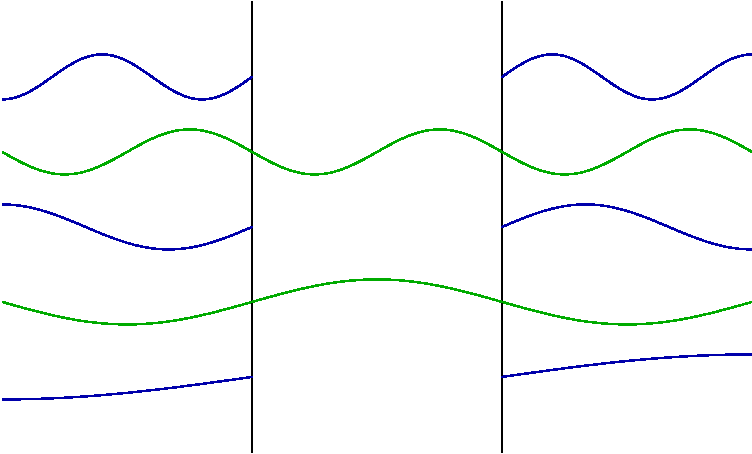
\includegraphics[width=6cm]{fig/intro/twoplanes_wave}
\caption[Allowed modes between parallel plates]
{Sketch of allowed modes between perfectly conducting plates. 
 Only waves with a half-integer number of wavelengths fit between the plates.
Blue modes are only allowed outside the plates, while green modes are allowed inside
and outside.  Modes have been vertically offset for clarity.  }
\label{fig:Casimir_sketch}
\end{figure}

The theory was extended by Lifshitz and coworkers to describe forces between dielectric half-spaces~\cite{Lifshitz1956,
Dzyaloshinskii1959,Dzyaloshinskii1961}.  This can recover the Casimir force between 
perfect conductors, and Casimir--Polder forces between atoms' and dielectric surfaces.  
We will sketch the derivation of the Lifshitz formula (which we will require later),
since this can naturally also compute the Casimir energy.

%  As intimidating as this expression is, it can be heuristically derived with
% relative ease via the ``argument principle''~\cite{vanKampen1968}.  
% In essence, since the Casimir energy is the sum of the vacuum energy over all modes, the energy can
% be written as a complex contour integral of the energy against a function with poles at the allowed 
% energies.  For two plates the allowed modes satisfy the Fabry-Perot condition,
% \begin{equation}
%   \Delta = 1 - r_1r_2 e^{2ik d}.
% \end{equation}


\subsubsection{Derivation of Lifshitz Formula}
\label{sec:lifshitz}
The Lifshitz formula for the Casimir energy can be found with an ingenious argument due to van Kampen\etal\cite{vanKampen1968}.
In its full generality, the Lifshitz formula gives the total energy for two planar dielectric bodies with dielectric constants $\epsilon_1,\epsilon_2$
separated by a medium with dielectric constant $\epsilon_3$.  
(This derivation parallels those is taken from \S 7.2 in Milonni~\cite{Milonni1994} and Ch.12 of Bordag\etal\cite{Bordag2009}.
A similar result emerges from the scattering approach as discussed by Lambrecht\etal\cite{Lambrecht2011}.)
The energy for the EM field in its ground state is 
\begin{equation}
  E = \sum_{\zeta}\sum_{k_x,k_y,\omega} \frac{\hbar\omega_k}{2},
\end{equation}
where the sum runs over all of the allowed modes for the particular arrangement of bodies.  
In this case, the  non-zero contribution to the Casimir effect comes from surface plasmon modes, which propagate along the interfaces
and decay exponentially away from the bodies.  
The sum over frequencies can be recast as a contour integral over complex frequency $\xi$, against a function $\Delta^{(\zeta)}$,
 whose poles occur at the allowed frequencies, with residue $\omega_k$:  
\begin{equation}
  E = \frac{L^2}{(2\pi)^2}\sum_{\zeta}\int_0^\infty dk_T\,k_T\oint d\xi\, 
  \frac{\hbar \xi}{2} \frac{1}{(2\pi i)\Delta^{(\zeta)}(\xi)}\frac{d\Delta^{(\zeta)}(\xi)}{d\xi},
\end{equation}
where the function $\Delta'(\xi)/[2\pi i\Delta(\xi)]$ is designed to have unit residue at the zeroes of $\Delta(\xi)$, 
and $k_T$ is the transverse wavenumber.  The factor of $L^2$ is accounted for by considering the energy 
per unit area.  
The energy can be simplified by integrating by parts leading to 
\begin{equation}
  \frac{E}{A} = \frac{\hbar}{16\pi^3 i}\sum_{\zeta}\int_0^\infty dk_Tk_T\oint d\xi \, \ln\Delta^{(\zeta)}(\xi).
\end{equation}
The most important modes are the surface modes, since these modes are sensitive to the position of the other body, where
these modes exponentially decay between the bodies.
The allowed frequencies for these modes must satisfy 
\begin{equation}
  r^{\zeta}_{13}r^{\zeta}_{23} e^{-2k_z d}=1,
\end{equation}
where $r^\zeta_i$ are the reflection coefficients for surface $i$ and polarization $\zeta$ and\
the wavenumber is given by $k_z=\sqrt{k_T^2-\epsilon(\omega)\omega^2/c^2}$.  The reflection coefficients
are given by 
\begin{equation}
  r\supTE_{13} = \frac{k_{z,1}-k_{z,3}}{k_{z,1}+k_{z,3}} \qquad 
  r\supTM_{13} = \frac{\epsilon_3k_{z,1}-\epsilon_1k_{z,3}}{\epsilon_3k_{z,1}+\epsilon_1k_{z,3}}.
\end{equation}
The frequency condition is suggestive of the requirement that accumulated round-trip phase 
(including reflections from both walls) is unity for
allowed modes (this interpretation is bolstered by considering the Casimir force between mirrors~\cite{Genet2003}).
This suggests choosing $\Delta(\xi) = 1-r^{\zeta}_{13}r^{\zeta}_{23} e^{-2k_z d}$, where the wavenumber $k_z$
and the reflection coefficients are functions of $\xi$.  

The complex contour integral can be split into two pieces: the integral over the right semi-circle 
is apparently independent of $d$, and can be ignored.  This leaves the integral along the imaginary 
frequency axis, $\omega=is$.  
It turns out Casimir effects are most naturally discussed along the imaginary frequency axis.  
Due to the causal nature of the dielectric response functions, the dielectric function is a 
smooth, real function on the imaginary axis.  This also means that the $z$-wavenumber is also real,
with $k_z=\sqrt{k_T^2+\epsilon(is)s^2/c^2}$, 
and that oscillatory functions like plane wave factors are replaced with real, decaying exponentials.  
Both of these features are extremely attractive for numerical methods, and so this is also
often used in numerical methods~\cite{Johnson2011}.

The Casimir energy between two dielectric half-spaces of permittivities $\epsilon_1, \epsilon_2$
separated by a gap of thickness filled with permittivity $\epsilon_3$ is given by 
\begin{align}
\frac{E}{L^2} =& -\frac{\hbar}{2\pi^2c^3}\int_0^\infty ds\, s^2 \epsilon_3
\int_1^\infty dp\,p\sum_{\zeta=\text{TE, TM}}\log\left[1 - r^{(\zeta)}_{13}r^{(\zeta)}_{23}e^{-2\sqrt{\epsilon_3}ps d/c}\right],
\label{eq:lifshitz}
\end{align}
where the electromagnetic reflection coefficients are given by 
\begin{align}
  r\supTE_{ij}  = \frac{\kappa_i-\kappa_j}{\kappa_i+\kappa_j},\quad
  r\supTM_{ij}  = \frac{\epsilon_j \kappa_i - \epsilon_i \kappa_j}{\epsilon_j \kappa_i + \epsilon_i \kappa_j},
\end{align}
and
\begin{equation}
  \kappa_i = \sqrt{p^2 + \epsilon_i/\epsilon_3-1}.
\end{equation}
following Zhou~\cite{Zhou1995}.
The variables have been adjusted to agree with Lifshitz original calculation, by defining 
\begin{align}
  k_T &= \frac{s}{c}\sqrt{\epsilon_3(p^2-1)}.
\end{align}
In general, this integral form is the simplest expression for the Casimir energy between dielectrics. 
% As intimidating as this expression may be, it is a necessary touchstone for later comparison, and it allows 
% us to examine the different scaling regimes at different distances.  
The perfect-conductor Casimir energy result (\ref{eq:Casimir_energy}) can be found by taking the strong-coupling limit,
 $r^{(\zeta)}_i\rightarrow 1$, and setting $\epsilon_3=1$.  and evaluating the integrals using 
\begin{equation}
  \int_0^\infty ds\,s^2 \int_1^{\infty} dp\,p \log[1 - e^{-2 s p d/c}] = -\frac{c^3 \pi^4}{360 d^3}.
\end{equation}
The Casimir--Polder results for interacting atoms can be recovered from the Lifshitz formula by taking the limit of dilute bodies,
$\epsilon \approx 1+\alpha n$, where $n\ll 1$ is the density, and $\alpha$ is the polarizability.

% This was further expanded on by Dzyaloshinskii\etal\cite{Dzyaloshinskii1959,Dzyaloshinskii1961} who
% showed the connection between Casimir force and the pair-wise van der Waals potentials.  
%This work is reviewed by McLachlan~\cite{McLachlan1963, McLachlan1963a}.  

The Lifshitz theory can be extended to account for dispersion and finite temperature.  
Some care is required in quantizing the electromagnetic field within dielectric media,
since due to the Kramers-Kr\"onig relations, the presence of dispersion implies dissipation.
% The usual approach to open-systems in quantum mechanics is to couple the system to a reservoir, 
% and integrate out the reservoir.  
However, it has been phenomenologically observed that one gets the correct answers by a direct substitution
$\epsilon(\vect{x})\rightarrow \epsilon(\omega,\vect{x})$.  This issue has in investigated more carefully in~
\cite{Barash1975,Rosa2010}, and justified by careful examination of the thermodynamic energy
and relation to the microscopic details of the medium.   

At non-zero temperature it is necessary to also include the effects of real thermally excited photons,
by accounting for the mean number of excited photons.
At inverse temperature $\beta=(\kB T)^{-1}$, for a 
frequency $\omega$, the mean number of photons is $\bar{n}(\omega) = \coth(\beta\hbar \omega/2)$.  
Note that $\coth(i x)$ has simple poles at $x=\pm n \pi$ for $n$ integer. 
Exactly the same style of argument can be used to find the thermal Casimir energy between dielectrics, 
but now due to the presence of $\coth(is)$, the integral over imaginary frequency picks up the residues of the integrand at the 
Matsubara frequencies $s_n:= 2\pi n/(\beta\hbar)$.
The resulting free energy per unit area is 
\begin{align}
  \frac{\mathcal{F}}{L^2} =& \frac{\kB T}{2\pi}{\sum_{n=0}^\infty}' s_n^2 \epsilon_3
  \int_1^\infty dp\,p\sum_{\zeta=\text{TE, TM}}\log\left[1 - r^{(\zeta)}_{13}(is_n)r^{(\zeta)}_{23}(is_n)e^{-2\sqrt{\epsilon_3}ps_n d/c}\right],
  \label{eq:lifshitz_finite_temp}
\end{align}
where the primed sum gives half the weight to the $n=0$ term, and all functions of frequency are evaluated at $s_n.$ 
At zero temperature, this result passes over to the previous one, 
by transforming the sum over frequencies into an integral.  This is the most general form of the Lifshitz
formula, and can recover all of the limiting behaviors at close distance, far field, and perfect conducting
media, and rarefied media.

\subsection{Physical Interpretation}

Casimir's original calculation vividly shows the importance of vacuum fields, and is said to show the reality 
of the vacuum field.  This is due to the emphasis given to the imposed boundary conditions,
which are emphasized over the matter that created the boundary conditions~\cite{Jaffe2005}.  
It is the author's opinion that the Casimir effect is best thought of as a long-ranged interaction between dielectric bodies 
mediated via the electromagnetic field~\cite{Jaffe2005, Rahi2009}.  This picture is also
analogous to the intuitive photon exchange picture used to explain the Casimir--Polder potential.
% This view makes the clearest connection to the underlying fundamental physics, rather than emphasizing idealized
% boundary conditions.
  Fig.~\ref{fig:electron-effective-interaction} shows a term contributing to the Casimir effect where 
electrons on different bodies interact with one another via the electromagnetic field.
  The solid lines should
be understood as the current operators for the electrons bound to a particular, separate media, while the 
wavy lines are the EM green functions describing the photon.  In fact, if summed over all such dipole ``bubbles'',
one can recover the full Casimir force results --- as was done by Dzyaloshinskii\etal in re-summing a field 
theoretic expansion~\cite{Dzyaloshinskii1961}.  
In that case the closed electron loops should be understood as current-current correlation functions,
$\langle j_\mu j_\nu\rangle$, where under linear response theory, this correlation function is related to the conductivity
tensor $\sigma_{\mu\nu}$~\cite{Kubo1957,Altland2011}.  The conductivity tensor is in turn related to the dielectric tensor, $\epsilon_{ij}$
via Ohm's Law $j_i=\sigma_{ij}E_j,$ which makes the connection between this condensed matter physics,
and the material functions used in the Casimir effect\footnote{
  This relationship was pointed out by Rahi\etal\cite{Rahi2009}, as a justification for their starting point
  in quantizing the electromagnetic field in media.}.

%\todo{Details of Kubo?}
% \comment{Effective interaction: expanding out perturbation theory leads to $\langle j_\mu j_\nu\rangle$
% correlation functions.  Via Kubo formalism for linear response, this is related to the conductivity
% tensor $\sigma_{\mu\nu}$, which is in turn related to the dielectric constant $\chi$}

 \begin{figure}
 \centering
 \begin{fmffile}{wall-wall}
% \begin{fmfgraph}(50,30)
%  \fmftop{t0,t1,t2,t3}
%  \fmfbottom{b0,b1,b2,b3}
%  \fmf{fermion,tension=0.5}{t1,v1}
%  \fmf{fermion,tension=0.5}{t2,v3}
%  \fmf{fermion,tension=0.5}{b1,v2}
%  \fmf{fermion,tension=0.5}{b2,v4}
%  \fmffreeze
% \fmf{photon,tension=0}{v1,v3}
% \fmf{photon,tension=0}{v2,v4}
% \fmf{fermion,tension=0}{v1,v2}
% %\fmf{fermion,tension=0,left}{v2,v1}
% \fmf{fermion,tension=0}{v3,v4}
% %\fmf{fermion,tension=0,right}{v4,v3}
% \end{fmfgraph}
\begin{fmfgraph}(50,30)
 \fmftop{t0,t1,t2,t3}
 \fmfbottom{b0,b1,b2,b3}
 \fmf{phantom}{t1,v1}
 \fmf{phantom}{t2,v3}
 \fmf{phantom}{b1,v2}
 \fmf{phantom}{b2,v4}
 \fmffreeze
\fmf{photon}{v1,v3}
\fmf{photon}{v2,v4}
\fmf{fermion,tension=0}{v1,v2}
\fmf{fermion,tension=0,left}{v2,v1}
\fmf{fermion,tension=0}{v3,v4}
\fmf{fermion,tension=0,right}{v4,v3}
\end{fmfgraph}
\end{fmffile}
\caption[Casimir Energy in terms of fundamental QED processes. ]
 {Casimir Energy in terms of fundamental QED processes.  The electrons are considered bound within their respective media,
 but still interact with electrons on other bodies by exchanging photons.  Any self-interactions are removed 
by renormalization via considering energy differences.  The effective interaction of the 
electron current with the field is described by the dielectric constant.}
\label{fig:electron-effective-interaction}
\end{figure}

\subsection{Comparison with other forces}

Casimir or van der Waals forces, are the dominant forces for electrically neutral bodies.  
However, they can be screened by other electrostatic forces in some circumstances, particularly if one is 
considering metal bodies~\cite{Lamoreaux2011,Bordag2009}.  
These electrostatic forces typically have a longer ranged force law than the Casimir effect, 
with a similar order of magnitude. 
In order to detect the classic Casimir force between conducting bodies, it is then necessary to carefully 
remove any stray background fields.  These arise from patch potentials (localized distributions of electric charge
on a conductors surface), stray charges, or adsorbed atoms.  

Note that while these electrostatic forces can be mitigated, the Casimir effect cannot be removed.  
The resulting power law potentials are relatively short-ranged power laws compared to the Coulomb potential 
between charged particles which decays $d^{-1}$. 
We will compare the size of the Casimir force to typical Coulomb energies that arise in experiments.
We will also compare the Casimir--Polder energy to the typical trapping potentials used to trap atoms.
  
% While the Casimir effect is short-ranged compared to the $d^{-1}$ Coulumb potential between charged particles.
% However, most bodies are electrically neutral and thus have no long-ranged Coulomb potential, whereas
% the Casimir effect applies even if the bodies have no net charge.  

For macroscopic bodies we can compare the Casimir energy for perfect 
metal conductors at a distance $d$ to the energy stored in the capacitance.
The Casimir pressure (force per unit area) is $P_{\text{Cas}}=\frac{\hbar c\pi^2}{240 d^3}$.
This can be can be compared to the energy in a parallel-plate capacitor (pg. 219 of \cite{Milonni1994}.)
For a parallel-plate capacitor, with surface charge density $\sigma$, the attractive force 
between the plates is $P_{\text{cap}}=\sigma^2/(2\epsilon_0)$.  For a parallel-plate capacitor filled with
vacuum, the capacitance is $C=A\epsilon_0/d = QV$, which implies $\sigma=Q/A=\epsilon_0V/d$.
The capacitive pressure is then $P_{\text{cap}}= \dfrac{\epsilon_0 V^2}{2d^2}$.  At a distance of $1\mu$m
this corresponds to a voltage of $17$mV.  
In experiments, voltages of this magnitude are observed from electrostatic sources~(Ch 18 and 19 of Ref.~\cite{Bordag2009}).

For conducting bodies, such stray potentials can emerge from variations in the work function
of the metal~\cite{Lamoreaux2011}.
If the Fermi surface dips below the surface of the metal, a localized electric charge can build up.
This is one of the dominant backgrounds in Casimir experiments, and must be subtracted off to extract the Casimir effect.
These various electrostatic potentials are randomly distributed and show a $d^{-1}$ power law
contribution to the force~\cite{Sushkov2011}, as opposed to the faster $d^{-2}--d^{-3}$ behavior expected
from the Casimir force.  

The typical Casimir--Polder energy scale can be estimated from dimensional considerations.
For a typical atom, with size $r=1\AA$, the dipole moment $d\sim er$.  The static polarizability
is then $\alpha\sim \sum_jd_j^2/(\hbar\omega_j)$.
The Casimir-Polder energy in the far-field is then
\begin{align}
  V\subCP &= -\frac{3\hbar c\alpha_0}{32\pi^2\epsilon_0 d^4}%\\
%  &= -\frac{3\hbar c e^2r^2}{32\pi^2\epsilon_0 \hbar\omega_0d^4}\\
%  &= -\frac{10^8 10^{-19}10^{-20}}{10^2  10^{-11} 10^{15}10^{-24}} eV\\
%  &= -\frac{10^{-31}}{10^{-19}} eV\\
  \approx -10^{-12}eV,
\end{align}
which corresponds to a frequency shift on the order of $10$kHz for a generic atom at 1$\mu$m.  
% In the near-field, it is necessary to shift over to the van der Waals energy, where the atom interacts
% with its image dipole.
In comparison, a far-off resonant light beam can create an all optical trap with a depth of $10^{-9} eV$
\footnote{Assume the atom is cooled down to the Doppler temperature, for which $E\sim\hbar\Gamma\sim 10^{-28}J\sim 10^{-9}eV$}
So at a distance of $1\mu$m from a surface, it may be possible to trap an atom, but at a tenth of that distance the Casimir--Polder
attraction would overcome the optical trapping potential.

%As comparison, a typical trapping potential using far detuned lasers is 
% As an example, atoms near a conducting surface can adsorb onto the surface, and form ionic bonds with a large dipole 
% moment.  This permanent dipole polarizes the atom, leading to an atttractive potential~\cite{McGuirk2004}.  
% The resulting potential can be written in terms of the atomic polarizability $\alpha$,
% \begin{equation}
%   V_{\text{ad}}(\vect{r}) = -\frac{\alpha_0}{2}|\vect{E}(\vect{r})|^2,
% \end{equation}
% where $\vect{E}$ is the field from the adatom dipole.  
% The electric field for a dipole at the origin of dipole moment $\vect{d}$ is 
% \begin{equation}
%   \vect{E}(\vect{r})=\frac{1}{4\pi\epsilon_0|\vect{r}|^3}[3(\vect{d}\cdot \hat{r})\hat{r}-\vect{d}]. 
% \end{equation}
% The square of the electric field is 
% \begin{equation}
%   |\vect{E}(\vect{r})|^2% =\frac{1}{(4\pi\epsilon_0|\vect{r}|^3)^2}
%   % [9(\vect{p}\cdot \hat{r})^2-6(\vect{p}\cdot\hat{r})^2+\vect{p}^2]
% =\frac{1}{(4\pi\epsilon_0|\vect{r}|^3)^2}  [3(\vect{d}\cdot \hat{r})^2+\vect{d}^2]
% \end{equation}
% So for order of magnitude estimates, the interaction potential is approximately
% \begin{equation}
%   V_{\text{ad}}(\vect{r}) \sim -\frac{\alpha_0}{2}\frac{1}{(4\pi\epsilon_0|\vect{r}|^3)^2}\vect{d}^2
% \end{equation}

\subsection{Different Distance Scaling Regimes}

The Casimir effect is important at distances around the resonant wavelengths of the atom or medium,
 which are typically on the order of $1\mu$m for optical transitions.  
The Casimir effect is typically computed in a long-wavelength or low energy limit where the constituents of the bodies can be treated 
as a continuum.
%This long-wavelength limit also corresponds to energies small compared to the binding energies of the bodies.
This approximation starts to break down when the distances between bodies approach the separation of the constituent atoms.
which is around $1\AA$, where exchange effects and other physics becomes important.
At the other limit, for distances beyond $100 \mu$m, the Casimir effect becomes too weak to detect.  

The distance scaling of the Casimir energy for bodies separated by a distance $d$, can be found by approximating 
the Lifshitz integral~(\ref{eq:lifshitz_finite_temp}) in certain limits.
%The differing scaling emerges by approximating the integrals in the Lifshitz formula~(\ref{eq:lifshitz_temperature}) in various limits.  
% The distance scaling depends on the nature of the bodies, and the how large the separation is in comparison to 
% relevant wavelengths in the problem.  
% For pairs of macroscopic slabs the energy scales as $d^{-2}$--$d^{-3}$, depending on the separation, 
% while the energy scales as $d^{-6}$--$d^{-7}$ for pairs of atoms.  
In particular, one must compare the separation of the bodies $d$ to the resonant wavelengths or frequencies of 
 of the interacting media.  
This requires some knowledge of the peak frequencies $\omega_A$ of the atomic polarizabilities $\alpha(\omega)$ or the dielectric
 function $\epsilon(\omega)$.  At nonzero temperature, there is another distance scale given by the thermal wavelength,
 $\omega_T=\kB T/\hbar$.  One can estimate the most important frequencies by examining $\alpha(is),\epsilon(is),e^{-2pd\xi/c}$
and approximating the integral in various limits. 

 In the near field or van der Waals regime, the separation of the bodies is less than any of the 
 resonant wavelengths for the bodies $d\ll \omega_A/c,\omega_M/c$.  In that limit $\epsilon(i\omega)$ serves to cut off 
 the frequency integral, and the exponential factor $e^{-2pd\xi/c}$
 is unity for all relevant frequencies.  In essence, the interaction is an instantaneous 
 dipole interaction between the media.  For example the atom-wall potential shows a $d^{-3}$ scaling. 

 In the retarded or Casimir-Polder regime, the atoms are much further than a resonant wavelength 
 $d\gg \omega_A/c,\omega_M/c$.  In that case the dominant contributions come at zero frequency, 
and the functions can be approximated with their static limit.
 This typically occurs for distances greater than a micron.
 In this far field regime, the potential typically decays more quickly.  For example, the  atom-wall
potentials shows a $d^{-4}$ scaling in this limit.

At even greater separations between the bodies is the thermal regime $d\sim \omega_T/c$, where the real photons excited by the 
 thermal field contribute significantly to polarizing the atom.  At room temperature, the thermal wavelength is
 $\lambda_T=\hbar c/(\kB T)~10\mu m$.  In this regime the potential falls off more slowly as $E\sim d^{-3}$,
 the same as the near-field van der Waals regime.  

\section{Overview of Casimir Experiments}
\label{sec:expt_review}

The Casimir effect has been measured in experiments, both for macroscopic bodies and atoms.
This section provides a brief overview of the broad categories of experiments where the Casimir effect is relevant,
and the challenges these experiments provide to theoretical and computational methods.    
The following is intended as a broad survey, since the full literature on the Casimir and Casimir--Polder 
effects is quite large.  

%Lamoreaux
\subsection{Experiments on Casimir Forces}

%\todo{Citation for this?}

Despite it's prediction in 1948, the Casimir effect proper proved quite difficult to directly measure.
Some early confirmations used the Casimir effect to explain the thickness of liquid helium film on 
the wall of its container~\cite{Sabisky1973,Dzyaloshinskii1961}.
In that case, helium satisfies the repulsive Casimir criterion and it is energetically favorable
to have helium between the vacuum and the walls.  
% An early indirect measurement was liquid Helium flowing up the walls of a container.  \todo{Citations!  Lifshitz/Dzyaloshinskii}
% Lifshitz and co-workers applied the Casimir pressure to explain the phenomenon of liquid helium
% flowing out of a jar.  
% The presence of the liquid helium crawling up the surface reduces the Casimir energy,
% between the vacuum and the sides of the jar, so the liquid helium experiences an attractive pressure up the walls.  

The Casimir effect was only precisely measured in 1997 by Lamoreaux~\cite{Lamoreaux1997}.   
%Lamoreaux's work spurred a large amount of experimental and theoretical work.  
This experiment measured the Casimir force between a sphere above a metal plate,
and measured the force via a torsion pendulum.  
This landmark experiment was closely followed by measurement by Mohideen\etal\cite{Mohideen1998}
using an atomic force microscope to measure the force in a sphere-plate geometry.  
The Casimir force has also been directly measured in a nanoelectromechanical (NEMS) system 
by Chan\etal~\cite{Chan2001}.  In this case, the Casimir force is detected by the modification it
makes to the frequency of a torsional oscillator suspended above a plate.  
The sphere-plate and oscillator geometries have the experimental advantage of removing the need to carefully
align the parallel metal plates. % Given the strength of the Casimir force it is hard to keep the plates exactly parallel,
% and separate, which is something that dogged early attempts to measure the Casimir force.
Despite the aforementioned difficulties, the Casimir force between parallel plates was measured precisely by Bressi\etal~\cite{Bressi2002}.  

The Casimir force is also important in applications of microelectromechanical systems (MEMS), 
as a source of stiction~\cite{Tas1996, Serry1998, Buks2001}.  This is particularly important
in free standing structures such as nano-oscillators.  %\todo{Comment on non-linear actuation blah?}
Given the Casimir force is an attractive potential, if parts of the device get too close to the substrate
they will permanently stick to one another, leading to device failure.  

Precisely measuring such a small force requires careful calibration of the measurements 
and removing systematic effects.  Reviews of these and other difficulties are available in Refs~(\cite{Lamoreaux2011, vanZwol2011, Bordag2009}).
Two of the primary experimental errors are due to 
patch potentials, and surface roughness.  The patch potentials are localized surface 
charge distributions, which due to the longer range Coulomb interaction must be subtracted off to extract the weaker
Casimir force~\cite{Sushkov2011}.  The fact that the thin metallic films and surfaces used in these 
experiments are not perfectly smooth is referred to as surface roughness, and is one of 
the main theoretical sources of error in these experiments.  
In addition, the optical properties of the surface must also be carefully characterized, since the 
optical properties of a coating can vary significantly.  Another difficulty in predicting the size of the 
Casimir effect is that the optical properties must be interpolated from data for other experiments~\cite{vanZwol2011}.

\subsection{Experiments on Casimir-Polder Forces}

Van der Waals and Casimir--Polder forces were first observed experimentally in molecules, 
which prompted the further development of theory to explain the effects.  
Beyond those early experiments, Casimir--Polder forces have also been measured precisely in more modern experiments  
using isolated atoms in experiments using atomic beams, cavity QED, and Bose-Einstein condensates.  

The first modern attempts at directly measuring the Casimir-Polder force used atomic beams 
near surfaces.  Sukenik\etal made the first modern attempt to measure the Casimir-Polder force~\cite{Sukenik1993}.
Their experiment passed a hot beam of atoms through an optical cavity and attempted to detect
the effect by the small phase-shift induced on the atoms.  Unfortunately, their measurement 
was not definitive.
More recent experiments by Perreault\etal\cite{Perreault2005}, and Lonig\etal\cite{Lonij2009} succeeded in measuring
the Casimir-Polder force with atomic beams.  These experiments passed an atomic beam past grating and 
detected the phase-shift by atom interferometry.  

The Casimir-Polder effect has also been observed in the context of a Bose-Einstein Condensate (BEC)
of ultra-cold atoms~\cite{Harber2005,Obrecht2007}.  % The BEC allows for precise distance control,
% and can be used in atom interferometry to detect small phase shifts.    
The atoms are confined to a harmonic trap, and can be brought near to a surface to probe the Casimir
force, where the Casimir force acts to shift the oscillation frequency of the harmonic trap in a position
dependent manner.  % These experiments were able to measure the Casimir--Polder force in the thermal regime,
% vary the distance of the atoms from the surface from $1\mu m$ up to 10 $\mu m$
% This technique was able to measure the Casimir force in the thermal regime, which
% is often difficult since the force is weak at those distance, but was accessible here due to the stability of the BEC.
% In this case it was ``easy'' to  to observe
% the cross over between the Casimir-Polder and thermal regimes.

The Casimir-Polder force is also important in developing atomic technologies.  
Atoms are an attractive platform for a number of reasons:
Each atom of the same species is identical; 
atoms have readily accessible, well-defined transitions that can be used to control their motion
, internal state and interactions; and atoms
have internal states that are long-lived, which would be important in storing information.

In recent years there has been a concerted push to develop technology that retains the appealing features 
of cold atoms in an architecture that can be scaled up to having large numbers of addressable atoms
~\cite{Kimble2008}.  
% There is a large effort across many fields to harness quantum technologies to develop scalable 
% quantum devices for computation and simulation of quantum systems
The desire to get strong-coupling between the atom and light fields, addressable qubits, and a scalable
architecture has pushed groups towards developing atomic traps that capture atoms close to dielectric surfaces.  
In this limit, the Casimir--Polder force is the dominant force, which can only be partially mitigated
by using laser fields to generate repulsive potentials.
In designing these new devices it is essential to compute and account for the Casimir-Polder force
the atom's experience when brought close to the dielectric surface.  

One direction that has been pursued is the atom-chip~\cite{Folman2000,Schneider2003,Salem2010},
where atoms are trapped within a few microns of the surface via a combination of lasers and magnetic fields from wires embedded in
the surface.  %The atoms are typically trapped within a micron of the surface.  
In most applications the Casimir effect acts as a lower bound on how close bodies can be brought 
to each other, which in turn limits the coupling strength, as well as how small devices can be made.
In the atom-chip example bringing the atoms closer than a micron lead to most of the atoms escaping the 
trap~\cite{Lin2004}.

Another direction that has been pursued is strong coupling of atoms to light via cavity 
quantum electrodynamics (QED).  
Kimble's group is developing microscopic dielectric waveguides to allow trapping, addressing and strongly interacting with  
single atoms in a scalable manner~\cite{Alton2011, Hung2013, Goban2014}.  In more recent work,
the Casimir--Polder potential is explicitly accounted for as part of the trapping potential~\cite{Goban2014},
and must be precisely computed.

\subsection{Current experimental directions}

Beyond directly detecting the Casimir effect, experiments are also moving in some directions worth highlighting,
since they are quite challenging for the theory to handle.  

% \subsubsection{Thermal Force and Material Model}

% There is a long-standing dispute between experimentalists on the best model to describe the 
% metals used in Casimir experiments.  In particular, should the metallic bodies be described by 
% the Drude or Plasma models?  These models provide the following dielectric constants for metals,
% \begin{align}
%   \epsilon_{\text{Drude}} &= 1+\frac{\omega_p^2}{\omega(\omega+i\gamma)}\\
%   \epsilon_{\text{plasma}} &= 1-\frac{\omega_p^2}{\omega^2},
% \end{align}
% where $\omega_p$ is the plasma frequency and $\gamma$ is the dissipation rate.
% The Drude model is consistent with Maxwell's equations, but some earlier experiments fit the plasma model 
% better.  This is also entangled in another debate over the role of the thermal Casimir effect, in particular what happens
% to the zero-frequency term from the TE polarization?  The Drude model has a simple pole at zero frequency,
% while the plasma model 
% These mattes are more a problem of reasoning than lacking theoretical or computational technology.  

% \subsubsection{Controversies over model}

% There are a couple as-yet unresolved issues in Casimir physics.
% Two of the leading experimental groups disagree on the appropriate model for the dielectric constant
% of a realistic metal.  
% Furthermore, there is also disagreement


%  Thermal casimir force
% Sushkov\cite{Sushkov2011}.
% Fight in literature over exact model used to describe metals at finite temperature.
% Drude vs plasma model.  
%  Lamoreaux favors Drude model, Capasso/Mohideen favours plasma model.

\subsubsection{Repulsive Casimir Effects}

Given that Casimir effects tend to enforce lower bounds for how close bodies can approach each other,
there have been a push to search for repulsive Casimir effects.  This would allow open the possibility
of trapping particles, and allow much smaller devices to be constructed.  
Unfortunately, these prospects are somewhat limited, due to requiring rare material properties.
From the Lifshitz formula, the sign of the force changes sign if $r_{12}r_{23}<0$.
This implies Casimir repulsion should be possible if $\epsilon_1<\epsilon_3<\epsilon_2$ over a broad range of frequencies.
This was experimentally demonstrated for a gold sphere immersed in bromobenzene above a silica plate
by Munday\etal\cite{Munday2009}.  However, this is method is little help for Casimir forces between
identical materials.  

Alternatively, the Casimir force is also repulsive for combinations of dielectric and magnetic materials~\cite{Boyer1974}.  
Given the strength of electric interactions over magnetic interactions in atoms, this spurred interest
in exploiting materials with strong magnetic responses~\cite{Kenneth2002}.  
Since these are relatively rare, there was some interest in exploiting metamaterials (arrays of micropatterned circuits with
effective magnetic response at certain wavelengths~\cite{Pendry1999}).  However, this was shown to be ineffective
for Casimir applications since the underlying metallic dielectric response dominates for the most important long wavelengths.
The metallic response implies an attractive potential, with the result that the overall Casimir effect would be attractive~
\cite{Ianuzzi2003comment,Rosa2008,Pirozhenko2008,Yannopapas2009}.  

While the preceding discussion emphasized varying materials for Casimir applications, it may 
be possible to exploit similar ideas for repulsive Casimir--Polder effects~\cite{Milton2011,Milton2012},
since the atom responds to a narrower range of frequencies.  In the far-field, the attractive dielectric
response may dominate, it might be possible to engineer near-field repulsion.  
These require an anisotropic response from the atom, which might be possible in the excited state.

Another way towards repulsive effects is by varying the geometry of the bodies.  
For example, the Casimir effect is repulsive in certain regimes for an elongated needle above a hole in a conducting plate~
\cite{Levin2010,Rodriguez2013}.  However, in this example the repulsion is unstable. 
In fact, it seems that it is impossible to get stable levitation for similar bodies via Casimir forces alone~\cite{Rahi2010}.

\subsubsection{Searches for new physics}

The Casimir force is also important for speculative searches for new physics on the millimeter to micron
scale~\cite{Dimopoulos2003, Bezerra2011}.  Since the new physics must be relatively short-ranged, 
it is typically modeled with a Yukawa potential, $V_{\text{Yuk}}=\alpha e^{-\lambda r}/r$,
which models the interaction with a new massive particle.    
On the micron scale however, the Casimir effect is the dominant interaction between neutral bodies,
 and must be carefully subtracted in an experimental procedure.
 Experiments then look for deviations from the expected Casimir effect, which means that the 
theory and experiment must be good agreement with one another.  
This approach has already been used to exclude regions of the parameter space for the hypothetical
Yukawa interaction~\cite{Obrecht2007,Bezerra2011}.  
Experiments searching for modifications of gravity typically employ a thin gold layer over
a density modulation.  The gold layer provides a common short-ranged Casimir interaction, while the 
a density modulation allows measuring variations due to gravity~\cite{Sorrentino2009, Geraci2015}.
Given the difficulties in cleanly measuring the Casimir force, this even more ambitious program has yet 
to yield results.  

% \subsection{Chemistry/Helium/Geckos?}

% \begin{enumerate}
% \item Geckos use the Casimir force \cite{Autumn2002}.
% \item Military applications to mimic at human scale. Cite 2015 paper.   
% \end{enumerate}


\section{Computational methods for Casimir Effects}
\label{sec:numerical_review}

Modern experiments require theoretical and computational methods
for the Casimir force that can account for a wide variety of material responses, anisotropies
and the ability to handle arbitrary shapes.  
% Although the Casimir force was explored by theorists before precision experiments were available,
% the advent of precision experiments and new technologies has spurred developments in 
% theoretical and computational methods.
% While early work focused on highly symmetric geometries 
% of bodies such as parallel planar bodies~\cite{Casimir1948,Lifshitz1956} or spheres~\cite{Boyer1968}, 
% current experiments require calculations for arbitrary shapes and arrangements of bodies, 
% which have realistic material properties.  
% This is a difficult task since the Casimir effect is a broadband phenomenon, depending on the whole 
% range of frequencies.  Furthermore, it depends sensitively on the geometry of the bodies involved, 
% and one must carefully renormalize the results to avoid infinite answers.  
For a simple, symmetric geometry (like perfectly conducting planes we used in Sec.~\ref{sec:CP_calc})
it is possible to write down tractable analytical expressions for
the Casimir energy based on expanding the field in mode functions.
%   However for general geometries 
% such an expansion may not be possible, or converge well.
However, for completely general geometries these requirements force one to adopt a general 
numerical approach to computing Casimir forces~\cite{Johnson2011}.
We will discuss three of these methods: the proximity-force approximation (PFA), the scattering
or fluctuating surface current approach, and the worldline method.

(We will briefly note methods based on computing van der Waals energies in the static field limit,
by evaluating functional determinants for discrete spatial grids~\cite{Maggs2006,Pasquali2008}. This approach 
omits any time evolution of the fields, but it does offer a direct method of trying to evaluate the field path integral.
That work relied on direct spatial discretization to evaluate the functional determinants, which limits
the size of medium that can be considered.)



% \begin{enumerate}
% %\item Experiments spurred development of theory.  
% % \item Prior methods relied on mode-function expansion of fields, which is only possible
% % for simple geometries.  
% % \item Theory must account for material properties.  Surface roughness.  
% % \item Need general methods, tend to result in numerical integrals.
% % \item Crudest method available is the proximity force approximation.  
% % \item Analytical theory based on green function methods.  (Russian school, McLachlan, Schwinger)
% % \item Scattering approach.  
% % \item Worldline method.  
% \end{enumerate}

\subsection{Proximity Force Approximation}

The proximity force approximation (PFA) or Derjaguin approximation, is an uncontrolled approximation to
the Casimir force between generally shaped objects~\cite{Derjaguin1934,Blocki1977}.  
%\todo{Earlier citation is available}
The PFA treats each infinitesimal patch of the surfaces as if they were planar bodies,
and sums up the pair-wise interactions between different patches.
The PFA is assumed to be valid if the radius of curvature of the bodies $R$, is large relative to 
their separation $d$.  
For many years the PFA was the only practical general method of estimating Casimir forces in arbitrary geometries.
The PFA has the advantage of being straightforward to implement, and functions as an order of magnitude
estimate for the Casimir force for arbitrary geometries.
% It was used by Lamoreaux to estimate the Casimir force between the sphere-plate
% in his landmark experiments, where the radius of the sphere was indeed large compared to the separations explored. 

However it has some prominent limitations. First, it is only valid for vanishing curvature.
Second, the PFA assumes that the force can be found by integrating up
the pair-wise Casimir forces between each pair of surface patches.  This ignores the non-additivity
of the Casimir force.  Unlike the potential between electric charges where the total potential is
the sum of the pair-wise potential energies, the Casimir force for an arrangement
of bodies is not just the sum of the pair-wise energies.~(See \S{8.2} and \S{8.4} of \cite{Milonni1994})
As a crude justification, the Casimir energy involves the square of the electric field, which responds 
non-linearly as more bodies are added.  
% Finally, the PFA allows only for strictly attractive forces.  
% In contrast, the Casimir force can be repulsive, albeit under difficult to engineer circumstances 
% such as media with a strong magnetic response, or anisotropic media.
%\todo{PFA with frequency response for material?}

% \begin{enumerate}
% %\item Find first use?  Lamoreaux mentions usage.  Derjaguin?
% % \item Note problem with non-additivity. The PFA explicitly assumes that the force
% % can be found by adding up the pair-wise contributions from each surface patch.  
% % However, the Casimir force is a global phenomenon, and the total Casimir force
% % Useful if very limited curvature, or effectively approximate geometry as planar.  
% \item Only attractive.  (real electromagnetic casimir forces have possibility of 
% being repulsive, even if hard to realize in general.)
% \item ever extended to include material properties?
% \item Despite these limitations, the PFA is relatively straightforward to implement,
% and functions as an order of magnitude estimate for the Casimir force.  In the limit
% of vanishing curvature, the PFA converges to the correct Casimir force.  
% \end{enumerate}


\subsection{Scattering Approach}

The scattering approach is currently the only general method of computing 
electromagnetic Casimir forces between general media.  The scattering method 
is based on scattering techniques from classical electromagnetic theory and quantum mechanics~\cite{Rahi2009}.
%The roots of the scattering method in Casimir physics go back a number of decades.  
This method has been developed by a number of groups as an analytical method for general geometries~\cite{Emig2004, Lambrecht2006,
Kenneth2006, Emig2007,
MaiaNeto2008,Canaguier-Durand2012,Rahi2009}.  
% In Casimir physics, one is often interested in the scattered 
% EM field emanating from an object --- the renormalized interaction energies can be thought of as 
% emerging from this scattering.  
The Casimir energy can be written as 
\begin{equation}
  E = \frac{\hbar c}{2\pi}\int_{0}^\infty d\xi \log\det[\mathbb{M}\mathbb{M}^{-1}_{\infty}]
  \label{eq:scattering}
\end{equation}
where $\mathbb{M}$ is the scattering matrix describing scattering between the free modes of the electromagnetic
field induced by the presence of bodies, and $\xi$ is the imaginary frequency~\cite{Rahi2009}.
The energy is renormalized via $\mathbb{M}^{-1}_\infty$,
which is the scattering matrix as the bodies are removed to spatial infinity, this basically removes any
coupling between bodies and serves to remove any self-interactions. 
The indices of these matrices run over the labels of the possible modes (such as wavelength, polarization, mode origin for different bodies).
%Since different bodies have different shapes, it is necessary t be able to transform basis.  
Derivations similar to the argument principle used in Sec.~\ref{sec:lifshitz} can be applied to describe the scattering between modes,
--- instead of reflection coefficients for a surface, one considers the full scattering matrix for each body,
where matrix indices run over the labels (such as wavenumber, polarization) for the modes.
This has been applied for two-body systems such as realistic mirrors~\cite{Lambrecht2006}, surface roughness, 
and spheres and planes~\cite{Canaguier-Durand2012}.   
This subclass of these methods rely on scattering between mode functions suited to analytical expansions,
 and while they in principle offer a general purpose numerical method, 
the simulations may be slow to converge if the choice of basis functions is poorly suited to the actual
geometry required.  

The Johnson group at MIT has developed a formulation of the scattering method that is better suited to numerical 
applications for piece-wise constant media~\cite{Rodriguez2007,Rodriguez2007a, Rodriguez2009,Reid2009,Reid2011, Reid2013}.  
% Instead of describing the scattering from one mode into another, one can describe the scattering 
% locally at each patch of a surface.  
% The scattering between objects is described by coupling different surface patches together via the
% free-space Green functions.  
% This has justification from the Surface Integral Equations used in classical electromagnetism 
% ~\cite{Stratton1941}, and a variant on Green's theorem~\cite{Emig2004},
% where one can describe the field in each region by its free-space analogue, and couple it along the surface.
% (At the level of perturbation theory where the Casimir effect is computed, the photon Green function 
% can be described by its classical counterpart.)
% This method has also been able to leverage the development of classical EM solvers to the Casimir problem~\cite{Johnson2011}.
The fluctuating-surface-current formulation is a general method for computing Casimir
energies for piece-wise continuous linear dielectric and magnetic media~\cite{Reid2009,Reid2011, Reid2013}.  
In essence the method calculates the interaction between electric and magnetic surface currents 
on different bodies, mediated by the electromagnetic field.  Mathematically this is derived 
from a path integral for the electromagnetic field, where the fields are restricted to obeying EM boundary conditions at the 
surfaces via functional $\delta$-functions (simpler boundary conditions were handled in this fashion in
~\cite{Bordag1985,Li1991}).  The $\delta$-functions introduce fields 
bound to the surfaces, which can be interpreted as surface currents flowing to enforce boundary conditions.
After integrating out the EM field in the interior and exterior regions, 
these surface currents interact with one another via the electromagnetic Green function.
Since the method assumes piece-wise, homogeneous media and enforces EM boundary
conditions, it is the relatively simple homogeneous EM Green function that appears in these expressions.
These surface integrals are then discretized by splitting the surface into a finite number of patches.
All of the surface currents can then be integrated over, leaving a functional determinant analogous to Eq.~(\ref{eq:scattering})
where now the matrix elements $\mathbb{M}$ describe the coupling between different surface-patches induced
by the Green function.  

Numerically, this method comes down to computing the determinant of a large matrix, which is 
an intensive operation.  If a matrix has $N$ non-zero entries, the determinant for a dense matrix requires $\order(N^3)$ operations.
While it is possible to parallelize computing the determinant~\cite{Beliakov2013}, this is difficult.
However, for a sparse matrix system, it may be possible to make this relatively efficient 
and only require $\order(N\log N)$ operations~\cite{Reid2009}.
Since each frequency $\xi$ contributes independently, the integral over $\xi$ could be
trivially parallelized, but this may only offer relatively little parallelization for some problems.

The fluctuating-surface-current method has been used to 
for example describing the energy dependence of tetrahedral nanoparticles, capsules, and other  
geometries~\cite{Reid2009,Reid2011,Rodriguez2010}.  It has also been used to find cases 
where the Casimir force is repulsive due to geometric effects~\cite{Levin2010}, although the repulsion
is not stable~\cite{Levin2010,Rodriguez2013} .  
The scattering method has also been used in the design of atomic traps near dielectric waveguides, where the Casimir--Polder
force is an essential component of the trap~\cite{Hung2013}.  

As we noted, the scattering method is the only available general method for computing Casimir effects.
However, it is useful to have multiple methods with different computational properties
and biases, particularly when extending calculations to unexplored domains.  We now turn to the worldline
method which offers a very different picture and numerical method.  

\section{Path Integrals}
\label{sec:feynman_path_integral}
In order to discuss the modern methods of computing the Casimir effect it is necessary to introduce
the path-integral.  The path integral was originally developed by Richard Feynman as an alternative 
formulation of quantum mechanics~\cite{Feynman1948,Feynman1965}.
In the path integral, the probability amplitude for a particle to propagate from one position to another,
is given by the sum over \emph{all} possible paths between the points.
(In fact the path integral can be derived as the propagator from more traditional operator quantum mechanics~\cite{Sakurai1994}.)
Each path is weighted with a phase $e^{iS[x(t)]/\hbar}$ where $S[x(t)]$ is the classical action for the path.
For a free particle, the allowed paths are Brownian motions, or diffusive in nature.  

    Path integrals have been used extensively in a wide range of theoretical physics~\cite{Kleinert2012}.
    While offering an intuitive picture of quantum mechanics, they are much harder to use 
    than typical operator mechanics for anything other than the simplest problems~\cite{Feynman1965}.
    However, path integrals form a natural basis for quantum field theories, where they offer a relativistically covariant
    quantization procedure that naturally accounts for the gauge symmetries 
    that underlie the Standard Model of particle physics~\cite{Brown1994,Srednicki2008}.
    % In these field theoretic path-integrals, the integral runs over
    % all possible field configurations connecting the initial and final states, and some care is required
    % to handle the redundant degrees of freedom implied by gauge invariance~\cite{Faddeev1991}.

    Path-integrals have also been used in mathematics and statistics to describe stochastic 
    processes~\cite{Kac1949,Durrett1996, Karatzas1991}.  Rather than solving the Schr\"odinger equation, 
    this path integral is solves a diffusion equation --- this effectively passes over to ``imaginary time'',
    since after the Wick rotation which replaces, $t\rightarrow -i \tau$, the Schr\"odinger equation is a diffusion equation.
    This mathematical path integral weights each path by $e^{-S_{E}[x]}$, where $S_E$ is the real-valued Euclidean action for the path.
    In this form the path-integral has clearer convergence properties, 
    since the paths are weighted by real, decaying exponentials, as opposed to the oscillatory integrals
    in Feynman's path integral.  

    % The path-integral is one way to view stochastic processes, along side stochastic differential
    % equations and diffusion or Fokker-Planck equations. 
    % The path-integral is an infinite dimensional integral, which is the solution to an associated 
    % diffusion equation.  One can randomly sample from the 
    % dominant portions of the integral via Monte Carlo numerical methods.  These random sample paths can
    % in turn be described by a stochastic differential equations.  %\todo{Gardiner citation for SDE-> PDE}
        
    Path integrals underlie most of the work carried out in this thesis: we will use path-integrals
    to quantize the electromagnetic field, and the worldline method relies heavily on path integrals.
    In addition, we will use the connection between path-integrals and diffusion equations
    to verify analytically that the worldline path integral gives the correct results, and enhance our numerical
    calculations.  Considering their importance to this thesis, we will 
    now derive Feynman's path integral, which will serve as a prototype for all of the path integrals
    that follow.  (Our derivation follows the simple one given in Sakurai~\cite{Sakurai1994}.)
    % They have even been used in studying quantum chaos---the study of the quantum analogues 
    % of classically chaotic systems~\cite{Gutzwiller1990}.  In the semiclassical limit
    % where the classical action $S[x(t)]$ is large, the path integral for a chaotic system
    % can be approximated by only considering paths with periodic orbits.  %\todo{Gutzwiller trace formula citation}

    \subsubsection{Derivation of Feynman's Path Integral}

    Let us consider the quantum mechanical treatment of a particle in a time-independent potential $V(\vect{x})$, with Hamiltonian 
    \begin{equation}
      \op{H} =  \frac{\op{\vect{p}}^2}{2m} + V(\op{\vect{x}}),
    \end{equation}
    where the position and momentum operators obey the following commutation relations,
    \begin{gather}
      [\op{x}_i,\op{p}_j] = i\hbar\delta_{ij}\qquad      [\op{x}_i,\op{x}_j] = [\op{p}_i,\op{p}_j]=0,
      \label{eq:commutation}
    \end{gather}
    with resolutions of the identity,
    \begin{gather}
      I = \int d^Dx |\vect{x}\rangle\langle\vect{x}| = \int \frac{d^Dp}{(2\pi\hbar)^D} |\vect{p}\rangle\langle\vect{p}|,
      \label{eq:identity}
    \end{gather}
    and state overlap
    \begin{equation}
      \langle \vect{x}|\vect{p}\rangle = e^{i\vect{p}\cdot\vect{x}/\hbar}.
      \label{eq:overlap}
    \end{equation}

    In quantum mechanics, the amplitude for a particle starting at $x_i$ at time $t=0$, and propagating
    to $x_f$ at time $t$ is given by 
    \begin{equation}
      \langle x_f,t| x_i, t_0\rangle = \langle x_f| e^{-i\op{H}t/\hbar}|x_i\rangle.
    \end{equation}
    The amplitude to propagate from $x_0$ to $x_f$ can be developed into a path integral in a number of steps.
    First, split the evolution operator into $N$ pieces, and insert $(N-1)$ resolutions of the $\vect{x}$-identity 
    and $N$ resolutions of the $\vect{p}$-identity between    the pieces
    \begin{align}
      \langle \vect{x}_f,t_f| \vect{x}_i, t_0\rangle % &= \int \prod_{k=1}^{N-1} d^Dx_k 
      % \langle \vect{x}_f|e^{-i\op{H}\Delta t/\hbar}|\vect{x}_{N-1}\rangle
      % \langle \vect{x}_{N-1}|e^{-i\op{H}\Delta t/\hbar}|\vect{x}_{N-2}\rangle
      % \cdots \langle \vect{x}_1|e^{-i\op{H}\Delta t/\hbar}|\vect{x}_{0}\rangle\\
      &=\int \prod_{k=1}^{N-1} d^Dx_k \prod_{j=0}^{N-1} \frac{d^Dp_j }{(2\pi\hbar)^D}
      \langle \vect{x}_N|\vect{p}_{N}\rangle\langle\vect{p}_{N}|e^{-i\op{H}\Delta t/\hbar}|\vect{x}_{N-1}\rangle\nonumber\\
      & \hspace{0.5cm}\times\langle \vect{x}_{N-1}|\vect{p}_{N-1}\rangle\langle\vect{p}_{N-1}|e^{-i\op{H}\Delta t/\hbar}|\vect{x}_{N-2}\rangle
      \cdots \langle \vect{x}_1|\vect{p}_1\rangle\langle \vect{p}_1|e^{-i\op{H}\Delta t/\hbar}|\vect{x}_{0}\rangle
    \end{align}
    where $\Delta t:=t/N$, and we have introduced $x_N=x_f, x_0=x_i$. 
    At this point we can note the basic structure: the total amplitude for 
    the particle to propagate from $x_0$ to $x_f$ is the product of the amplitudes to propagate 
    from one point to the next, with the total amplitude being the integral (or sum) summed over 
    such paths.  
    Each infinitesimal time evolution operator can factored into a kinetic and potential piece, 
    \begin{equation}
      e^{-i\op{H}\Delta t/\hbar} = \exp\left(-i\frac{\op{p}^2}{2m\hbar}\Delta t\right)
      \exp\left(-iV(\op{x})\Delta t\right)+\order(\Delta t^2),
    \end{equation}
    where the corrections due to splitting and factorizing the exponential operator are higher order 
    in $\Delta t$.  
    (In general, it is crucial to consistently carry out all expansions in path-integrals to $\order(\Delta t)$.  
    % For example, in path integrals in curved space this often requires working to high order in $\Delta x$, 
    % and exploiting the equivalent of the Ito rule $dx^2=dt$~\cite{deWitt1957,Kleinert2012,Grosche1998}.
    )

    At this point, the position and momentum operators can be replaced by their eigenvalues, and the
    state-overlap can be used to write,
    \begin{align}
      \langle \vect{x}_f,t_f| \vect{x}_i, t_0\rangle 
      % &= \int \prod_{k=1}^{N-1} d^Dx_k \prod_{j=0}^{N-1} \frac{d^Dp_j }{(2\pi\hbar)^D}
      % \nonumber\\
      % \prod_{n=0}^{N-1}\bigg[\langle \vect{x}_{n+1}|\vect{p}_{n+1}\rangle
      % \langle\vect{p}_{n+1}|e^{-i\vect{p}^2_{n+1}\Delta t/(2m\hbar)}
      %   e^{-iV(\vect{x}_n)\Delta t/\hbar }|\vect{x}_{n}\rangle\bigg]\\
        &= \int \prod_{k=1}^{N-1} d^Dx_k \prod_{k=1}^{N-1} \frac{d^Dp_k }{(2\pi\hbar)^D}\nonumber\\
      &\times\bigg[\prod_{n=0}^{N-1}  e^{-i\vect{p}^2_{n+1}\Delta t/(2m\hbar)}     e^{-iV(\vect{x}_n)\Delta t/\hbar }
      e^{i(\vect{x}_{n+1}-\vect{x}_n)\cdot\vect{p}_{n+1}/\hbar}\bigg].
    \end{align}
    Since the momentum integrals are Gaussian, they can be straightforwardly evaluated
    \begin{align}
      \langle \vect{x}_f,t_f| \vect{x}_i, t_0\rangle 
      % &= \int \prod_{k=1}^{N-1} d^Dx_k \prod_{k=0}^{N-1} \frac{d^Dp_k }{(2\pi\hbar)^D}
      %   \prod_{n=0}^{N-1}\bigg\{  \exp\left[-\frac{i\Delta t}{2m\hbar}\left(\vect{p}_{n+1}  
      %       -\frac{m}{\Delta t}(\vect{x}_{n+1}-\vect{x}_n)\right)^2\right]\nonumber\\
      %   &\hspace{6cm}        \times \exp\left[ \frac{i m }{2\hbar\Delta t}(\vect{x}_{n+1}-\vect{x}_n)^2-\frac{i\Delta t}{\hbar}V(\vect{x}_n)\right]\bigg\}\\
        &= \int \prod_{k=1}^{N-1} d^Dx_k 
        \prod_{n=0}^{N-1}\bigg[\bigg(\frac{ m }{2\pi i\hbar\Delta t}\bigg)^{D/2}
        e^{i m (\vect{x}_{n+1}-\vect{x}_n)^2/(2\Delta t)}e^{ -iV(\vect{x}_n)\Delta t/\hbar}\bigg]\\
        &= \mathcal{N}\int D\vect{x} 
        \exp\left\{\frac{i}{\hbar}\int_{0}^{t} dt'\,\left[ \frac{m}{2} \dot{\vect{x}}^2-V[\vect{x}(t')]\right]\right\},
    \end{align}
    where in the final line we have taken the continuum limit, replacing $(\vect{x}_{n+1}-\vect{x}_n)/\Delta t
    \rightarrow \dot{\vect{x}}, \sum_n\Delta t f(n\Delta t) \rightarrow \int dt f(t)$, and introducing 
    $D\vect{x} = \prod_{k=1}^{N-1}d^Dx_k$.  The phase in exponent is the classical action for a particle
    in a potential.  Paths with the same phase will add together constructively, while 
    paths in regions where the phase is quickly varying will cancel one another out.  
    This leads to the classical limit where only the paths of stationary phase where $\delta S[x(t)]=0$
    contribute.

    % One can think of the integral as summing over all possible paths $\vect{x}(t)$
    % between points $x_0$ and $x_f$ weighted by their classical action.  This also suggests a number 
    % of semi-classical expansions, such as considering the limit when $\hbar\rightarrow 0$ to derive 
    % the classical limit, or in work on chaotic systems~\cite{Gutzwiller1990}.

    In this thesis, this simple type of derivation will be all we require.  We 
    will often work with the imaginary time version, which replaces the oscillating exponentials with
    decaying exponentials.  
    The extension to field path-integrals over fields is straightforward: the field $\phi(\vect{x})$ 
    is described by its value at finitely many points $\phi(\vect{x}_k)$, and one integrates over the field values at these 
    points.  At the end of the calculation, one lets the spacing between grid points go to zero, 
    and the size of the grid extend to infinity.  
    We will also only need to consider Gaussian path integrals, of the type considered here.  
    In a later chapter we will extend this derivation to include sources.

\section{Scalar Worldline Casimir Energies}
\label{sec:dirichlet_worldline}
The worldline method is an alternative method for computing Casimir energies.
The worldline method is a descendant of the scalar electrodynamics 
Feynman explored~\cite{Feynman1950}, where the effect of a quantum
field is described by summing over the paths of a virtual particle interacting with the other bodies. 
The worldline method was later developed as an alternative method for 
carrying out general quantum field theory calculations in terms of single particle 
quantum mechanics~\cite{McKeon1993, Strassler1992,Schubert2001}.  
% The worldline method is heavily based on Feynman's path-integral method, where the amplitude
% for a particle to move from one position to another is the sum over all paths between the positions,
% where each path acquires a phase proportional to the classical action for that path~\cite{Feynman1948,Feynman1965}.
The basic insight of the worldline method is that for one-loop effective actions, 
the field path integral calculation can be recast in terms of the particle path
 integral for particles traveling in closed space-time paths.
  Higher order loop calculations can also be carried out with more particles, 
and gauge fields can also be treated~\cite{Schubert2001}.
For example, the worldline method has been used to compute relativistic
field effects for quantum electrodynamics (QED) such as the Lamb shift~\cite{Schmidt1995},  
It has also been used as a numerical algorithm for computing these relativistic QED effects~\cite{Mazur2014}---
however, these methods were developed for free-space interactions at high energy, rather than the 
low energy Casimir phenomena we desire to describe.  

The worldline method was first used to compute scalar Casimir energies by Gies\etal~\cite{Gies2003,Gies2006, Gies2006a}.
The scalar worldline method has been extended to finite temperatures~\cite{Klingmueller2008},
 used to study the torsion of inclined planes~\cite{Weber2009},
and forces in the sphere-plane and cylinder-plane geometries~\cite{Weber2010, Weber2010a}.  
In these non-trivial geometries the worldline method has also been used to examine the failure of the proximity force approximation.
More recent work has focused on computing the stress-energy tensor~\cite{Schafer2012, Schafer2016},
with a view to exploring how the Casimir energy violates certain energy conditions (violations of which are required for certain exotic physics).

The scalar worldline is also related to some semi-classical expansions for the Casimir energy.  
In particular, it is a direct numerical method for computing the so-called optical path integral
\cite{Scardicchio2005, Scardicchio2006}.  The sum over intersecting paths is also reminiscent 
for the semi-classical approach to the Casimir force by Schaden and Spruch\cite{Schaden1998} that evaluates 
the Casimir energy by summing over all periodic orbits of light.  This latter work is particularly 
related to other work on the semiclassical limits of path integrals involving chaos~\cite{Gutzwiller1990}.
Both of these approximate techniques rely on a path integral expression for the Casimir energy that approximates electromagnetism as a
scalar field, and the worldline provides a general purpose way of evaluating those path integrals.   

The worldline method has also been applied to the Casimir piston, where there are interesting geometric effects
based on the geometry of the piston~\cite{Schaden2009,Schaden2009a}.
Most of this work is for idealized surfaces that imposed Dirichlet boundary conditions, but 
there has also been some effort to extend the worldline method to account for Neumann boundary
conditions~\cite{Fosco2010}.  To date there has only been speculation on how to extend the 
worldline method to electromagnetism~\cite{Aehlig2011}, which only considered perfect conductors,
and did not have concrete, correct results.    

% \begin{enumerate}
%   \item Semi-classical approach to Casimir force via trace formula~\cite{Schaden1998}
%   \item Also the optical path-integral.
% \end{enumerate}

% We consider a scalar field coupled to a background potential $V(\vect{x},t)$.  This potential
% embodies the location of the bodies we are considering.  % Starting from the classical action,
% we will derive the Hamiltonian for the fields, and then compute the quantum partition function.  
% The partition function can be written as a path-integral, which is readily evaluated as a functional
% determinant.  Ultimately we want the free energy, which can be further converted into a path integral
% for a fictitious single-particle.  This single-particle path integral forms the basis of the numerical
% world line method.   
\subsection{Derivation of the Scalar Casimir Worldline Path Integral}
We now introduce the basic scalar worldline method, to discuss its positive features and limitations. 
We will use terminology and scaling of dimensions in common with our later work, rather than the 
choices used in the original papers by Gies\etal~\cite{Gies2003}.

\change{See also Ch 20 of Steck's Quantum Optics notes for an alternative perspective on this work, including
some of the analytical techniques we will use later.}

(As a matter of convention we will distinguish between $\vect{r}$ as a position label or parameter
 and $\vect{x}$, the coordinate of a path integral)

Consider a scalar field $\phi(\vect{r},t)$, interacting with a background potential $V(\vect{r},t)$.  
The action for the field $\phi$ is given by 
\begin{equation}
  S = \int_0^T dt \int d\vect{r} \cL = \int_0^T dt \int d^{D-1}\vect{r} 
  \left[ \frac{1}{2c^2}(\partial_t\phi)^2-\frac{1}{2}|\nabla\phi|^2-V(\vect{r},t)\phi^2\right],
\end{equation}
where $V(\vect{r},t)$ defines the surfaces of the interacting objects
\begin{equation}
  V(\vect{r}) := \lambda \sum_r \delta[\sigma_r(\vect{r}-\vect{R}_r)],
\end{equation}
where $\lambda$ is the coupling constant, $\sigma_r(\vect{r})=0$ marks the locations of the surfaces, 
and $\vect{R}_r$ marks the center location of each body.
In most work on scalar worldlines, the coupling constant $\lambda$ is taken to infinity, 
which corresponds to imposing Dirichlet boundary conditions on the surfaces. 
For planar geometries, this recovers electromagnetic Casimir results for idealized perfect conductors.  

From the Lagrangian, one can find the Hamiltonian and quantize the theory.
% (While this is a somewhat length procedure, it is the clear formal procedure for quantization,
%  and useful to follow in cases where there may be ambiguities).
The momentum conjugate to $\phi$ is given by
\begin{equation}
  \Pi := \frac{\delta \cL}{\delta(\partial_t\phi)} = \frac{1}{c^2}\partial_t\phi,
\end{equation}
where $\frac{\delta}{\delta f(t)}$ denotes the functional derivative with respect to $f(t)$.    
The Hamiltonian is then given by
\begin{align}
  H &:= \int d^3r\,(\Pi\partial_t\phi -  L)= \int d^3r\,\bigg[\frac{\Pi^2}{2} + \frac{1}{2}(\nabla\phi)^2 +V(\vect{r},t)\phi^2\bigg].  
\end{align}
We are now in a position to quantize the theory by promoting the classical fields to quantum operators, 
$\phi\rightarrow \op{\phi},\, \Pi\rightarrow\op{\Pi}$.
The fields can be promoted to operators with equal-time commutation relations
\begin{equation}
  [\op{\phi}(\vect{r},t),\op{\Pi}(\vect{r'},t)] = i\hbar \delta(\vect{r}-\vect{r'}).
\end{equation}
In exactly analogous fashion to quantum mechanics, the overlap between states is given by 
\begin{equation}
  \langle \phi|\Pi\rangle = \exp\bigg[\frac{i}{\hbar}\int d^3r \phi(\vect{r})\Pi(\vect{r})\bigg].
\end{equation}

We can compute physical quantities of interest such as Casimir energies and forces
by taking suitable derivatives of the partition function. 
The quantum partition function for the field is 
\begin{equation}
  Z = \tr[ e^{-\beta\op{H}}] = \int d\phi \langle \phi| e^{-\beta \op{H}}|\phi\rangle,
\end{equation}
the trace is evaluated over the complete set of field states.  
It is actually more useful to carry out calculations with the free energy $\mathcal{F}=-\kB T \log Z$.
In classic path-integral fashion the exponential operator can be split into $N$ pieces, and resolutions of the identity
in both fields and conjugate-momentum fields can be inserted between each piece.  

% \begin{align}
%   Z &= \int d\phi_0\prod_{n=1}^N d\phi_n \langle \phi_n| e^{-\Delta \beta \op{H}}|\Pi_n\rangle
%   \langle\Pi_n| \phi_{n-1}\rangle
% \end{align}
After integrating out the momentum fields, the partition function can be written as a
Euclidean Path integral
\begin{equation}
  Z = \int D\phi \exp\left\{-\int_0^{\hbar\beta c} d\tau \int d^3r
    \left[ \frac{1}{2}(\partial_\tau\phi)^2+\frac{1}{2}(\nabla\phi)^2+V(\vect{r})\phi^2\right]\right\},
\end{equation}
where $\tau=\beta\hbar c$.  The partition function can be cast into a more suggestive form
by integrating by parts in the exponential integrand, 
\begin{equation}
  Z = \int D\phi \exp\left\{-\int_0^{\hbar\beta c} d\tau \int d^3r\,\phi(\vect{r},\tau)
    \left[-\frac{1}{2}\partial_\tau^2-\frac{1}{2}\nabla^2+V(\vect{r})\right]\phi(\vect{r},\tau)\right\},
\end{equation}
where the surface terms can be discarded by assuming the fields tend to zero at spatial (and temporal)
infinity.% \comment{Actually need frequencies for periodic functions.  Especially for finite temperature,
% dispersion.  Will discuss more carefully later.}

The functional integral over $\phi$ is Gaussian and can be formally evaluated immediately as a 
functional determinant, since the differential operator is positive operator.  
Some care is required in regularizing such infinite determinants.
This is done in analogy with finite dimensional Gaussian integrals.  
The fields can be considered as only being evaluated on a finite lattice of space-time points,
with the lattice also having a finite extent which bounds all bodies.  
The gradient operators can be treated via their finite difference approximations, 
which can be thought of as sparse matrices.
For example, $\partial_x^2\phi(x_k) \approx [\phi(x_k+\Delta)-2\phi(x_k)+\phi(x_k-\Delta)]/\Delta^2$
In that case the partition function is a large, finite Gaussian integral of the form, 
\begin{equation}
  Z_{\text{reg}} = \int d\phi_k\exp\left\{-\sum_{j,k}\Delta \tau (\Delta x)^{D-1}\phi_k A_{jk}\phi_j\right\}.
\end{equation}
where the labels over positions have been labeled with indices and the matrix $A$ represents the differential
operator.  
This regularized expression can be integrated, under the assumption that the eigenbasis of $A$ can be found, i.e.
where $A_{jk}\psi^{(n)}_k=\lambda_{(n)}\psi^{(n)}_k$.  In that case, each Gaussian integral decouples and the 
regularized partition function can be written as 
\begin{equation}
   Z_{\text{reg}} = C \prod_k \lambda_{(n)}^{-1/2} = C \det[A],
\end{equation}
where the determinant is understood to be the product of the eigenvalues of the operator $A$.
The limit of an arbitrarily large volume, and lattice resolution can be taken after integration.

In an analogous fashion, one can formally evaluate the partition function path integral as a 
functional determinant, 
\begin{equation}
  Z \propto {\det}^{-1/2}\left[-\frac{1}{2}\partial_\tau^2-\frac{1}{2}\nabla^2+V(\vect{r})\right].
\end{equation}
% The original computations for the worldline method stressed computing the quantum effective
% action for the scalar field.  This yields essentially the same expression.  This expression has
% also retained a factor of $2$ on the gradients --- this will simplify the representation of the 
% worldline path integral.
The proportionality is due to an additional (infinite) normalization constant, which will
be divided out in the renormalization process.  
The free energy for the interacting field can be written as 
\begin{equation}
  \mathcal{F} = -\kB T\log Z = \frac{1}{2}\kB T 
\log\det\bigg[-\frac{1}{2}\partial_\tau^2-\frac{1}{2}\nabla^2+V(\vect{r})\bigg]+C,
  \label{eq:free-energy-det}
\end{equation}
where $C$ is a constant.  
As it stands this functional determinant is divergent, but finite results can be found by subtracting off the 
free energy when the bodies are removed to spatial infinity.  Physically this corresponds to 
computing energy differences between different configurations of bodies.  % The renormalization also cancels off 
% the infinite constant normalization factors.  
The renormalized free energy can now be converted into a single-particle path integral via some formal 
manipulations.  First, we will use the identity $\log\det A=\tr\log A$, which can be readily
verified for positive finite matrices.  
\begin{align}
  \log\det A &= \log\prod_j \alpha_j
  =\sum_j \log\alpha_j
  = \tr\log A,\label{eq:log-det}
\end{align}
where we used the facts that the trace and determinant of a matrix are given by the sum
and product of its eigenvalues respectively. 
Second, the logarithm can be rewritten in an integral representation,
\begin{equation}
  \log A -\log B= -\int_0^\infty \frac{d\cT}{\cT} (e^{-A\cT} - e^{-B\cT}),\label{eq:integral_log}
\end{equation}
where $A$ and $B$ are positive operators (i.e. $A$ and $B$ have strictly positive eigenvalues).
This expression also relies on a difference of terms to cancel out divergent terms at $\cT=0$.  The 
earlier renormalization by subtracting off the vacuum energy provides exactly this subtraction. 

By applying Eqs.~(\ref{eq:log-det}) and (\ref{eq:integral_log}) to free energy~(\ref{eq:free-energy-det}),
 the renormalized free energy can be rewritten as
\begin{equation}
  \mathcal{F}-\mathcal{F}_0 = -\frac{\kB T}{2}\int_0^\infty \frac{d\cT}{\cT}
  \tr\Big[e^{[(\partial_\tau^2+\nabla^2)/2-V(\vect{x})]\cT}-e^{(\partial_\tau^2+\nabla^2)\cT/2}\Big].
\end{equation}
The trace can be evaluated by introducing a $D$-dimensional auxiliary Hilbert space, where 
$\langle \vect{x},x_{\tau}| \op{p}_i|\psi\rangle = -i \partial_i\langle \vect{x},x_{\tau}|\psi\rangle$,
$[\op{x}_i,\op{p}_j]=i\delta_{ij}$, with the result that 
\begin{equation}
  \mathcal{F}-\mathcal{F}_0 = -\frac{\kB T}{2}\int_0^\infty \frac{d\cT}{\cT}
  \int d\vect{x}_0d\tau_0 \langle \vect{x}_0,\tau_0|e^{-(\op{p}_\tau^2+\op{\vect{p}}^2)\cT/2 -\cT V(\op{\vect{x}})}-e^{-(\op{p}_\tau^2+\op{\vect{p}}^2)\cT/2}\big)
  |\vect{x}_0,\tau_0\rangle.
\end{equation}
The free energy is then in the form of the imaginary-time transition amplitude for a quantum particle
in $D$ space-time dimensions, in a potential $V$.
  In exactly the same fashion as Sec.~\ref{sec:feynman_path_integral},
this can be converted into a single-particle path integral, although 
there are some minor differences.  First, the starting and ending points are the same,
so the random paths form closed loops.  
Second, the time parameter $\cT$ is a fictitious parameter, with dimension of $L^2$, rather
than the physical time between events.
The resulting worldline path-integral for the free energy at zero temperature  is
  \begin{align}
    \mathcal{F}-\mathcal{F}_0 
    =&  -\frac{\kB T}{2}\int_0^\infty \frac{d\cT}{\cT}
    \int d\vect{x}_0  d\tau_0 \int \prod_{k=1}^Nd\vect{x}_k d\tau_k \nonumber\\
    &\times\prod_{k=0}^{N-1}\bigg[\frac{1}{(2\pi\Delta\cT)^{D/2}}
    e^{-(\vect{x}_{k+1}-\vect{x}_k)^2/(2\Delta \cT)}e^{-(\tau_{k+1}-\tau_k)^2/(2\Delta \cT)}\bigg]\nonumber\\
    &\times \bigg(\prod_{j=1}^Ne^{-\Delta\cT V(\vect{x}_j)}-1\bigg)\delta(\vect{x}_N-\vect{x}_0)
    \delta(\tau_N-\tau_0).
  \end{align}
The intermediate Gaussian integrals over $\tau_k$ can be carried out immediately, since the potential
is independent of $\tau$.  
The final integral $\int d\tau_0 = \beta\hbar c$, since $\tau_0\in[0,\beta\hbar c]$.  
% (A more careful derivation for non-zero temperature handles the $\tau$ direction via a Fourier transform,
% which introduces the Matsubara frequencies, $s_n = 2\pi n/(\beta \hbar)$.  
There is also a normalization constant of $(2\pi\cT)^{-1/2}$ for each dimension due to the loop 
closure condition.  This can be thought of as the total normalization for $N$ Gaussian steps of length 
$\Delta \cT= \cT/N$, subject to the loop-closure requirement $x_0=x_N$.
% The normalization can be understood from manipulations on the $\delta$-function, where 
% we require the multidimensional version of 
% \begin{equation}
%   \int dx \delta[h(x)]f(x) = \sum_{f(x)=0}\frac{f(x)}{|h'(x)|},
% \end{equation}
% which is given by
% \begin{equation}
%   \int \prod_{k=1}^Ndq_k \delta[h(\vect{q})]f(\vect{q}) = \oint_{h^{-1}(0)} dS\, 
%   \frac{1}{\sqrt{|\nabla_qh(\vect{q})|^2}}f(\vect{q}),
% \end{equation}
% where $\nabla_q h(\vect{q}) = \sum_i \frac{\partial h}{\partial q_i}$, and 
% the surface integral runs over coordinates satisfying the $h(\vect{q})=0$ condition~\cite{Hormander1983}. 
% If we change variable to $\Delta \tau_k = \tau_{k+1}-\tau_k$, then the loop closure condition is 
% \begin{equation}
%   \tau_0 - \tau_N = \sum_{k}\Delta \tau_k = 0.
% \end{equation}
The free energy can be written in a more intuitive form, better suited to numerical calculations,
if we consider the coupled Gaussians as the probability distribution for paths through space-time.
Each path increment $\Delta \vect{x}_k=\vect{x}_{k+1}-\vect{x}_k$ is Gaussian with zero mean and variance $\Delta \cT$.
In addition, the resulting paths must close on themselves --- such Brownian motions with fixed end points are 
referred to as Brownian bridges in the statistics literature~\cite{Karatzas1991}.  
The result of these manipulations is 
\begin{align}
  \mathcal{F}-\mathcal{F}_0 =& -\frac{\hbar c}{2}\int \frac{d\cT}{(2\pi\cT)^{D/2}\cT} \int d\vect{x}_0
  \dlangle e^{-\cT\langle V\rangle} - 1\drangle,
  \label{eq:scalar_worldline}
\end{align}
 where $\dlangle\cdots\drangle$ denotes an ensemble average over closed Brownian bridges $\vect{x}(t)$
starting at $\vect{x}_0$ and returning with $\vect{x}_N=\vect{x}_0$, and 
\begin{equation}
  \langle V\rangle := \frac{1}{\cT}\int_0^\cT dt\,V[\vect{x}(t)] = \frac{1}{N}\sum_{k=0}^{N-1}V(\vect{x}_k)
\end{equation}  
is the path-averaged value of the potential. 

The worldline method relies on generating an ensemble of closed Brownian bridges, and evaluating
the path-averaged potential for each path.  One must also integrate over the starting point $\vect{x}_0$
of the paths, and the path-time $\cT$.  The path-time $\cT$ governs the spatial extent of the paths, 
where the typical extent of is given by $x\sim\sqrt{\cT}$.
The renormalization against vacuum ensures that only paths that touch one of the bodies contribute.  
In order to extract interaction energies (such as the two-body Casimir energy) one subtracts off the 
one-body energies, which only account for the potential from one body.  As a result, only
paths that touch both bodies will contribute.  This is depicted in Fig.~\ref{fig:strong_coupling_cartoon},
where the upper path would contribute to the Casimir energy, while the lower path would not.  
At small times $\cT$, both paths would shrink down around their starting points, 
and since the paths would not touch both bodies, neither would contribute.
This is a direct result of the energy renormalization --- subtracting off
the vacuum energy cuts off the divergent $\cT$ integral as small $\cT$.  
At later times $\cT$, these paths would have larger extent, and both would contribute, but due 
to the $\cT^{-(1+D/2)}$ dependence, the lower-path would have a smaller contribution.  

The distance dependence can also be read off from Eq.~(\ref{eq:scalar_worldline}).  The typical extent of a Brownian motion of path-time
$\cT$ is $\sqrt{\cT}$. The average time a path touches the surface a distance $d$ away, is then $\cT\sim d^2$.
Since the integral is only non-zero after a path intersects the bodies, and the integrand is unit otherwise,
the energy density at a point $d$ from the surface is approximately $\int_{d^2}^\infty d\cT\, \cT^{1+D/2}\sim d^{-D/2}$.  
After integration over the starting point, one finds the Casimir energy scales as $d^{-3}$ in four
space-time dimensions.

\begin{figure}
\center
\includegraphics[width=10cm]{fig/intro/hit_strong_coupling}
\caption[Schematic of worldline paths interacting with plane and sphere]
{Schematic of worldline paths interacting with plane and sphere.  
  Only paths which touch \emph{both} bodies will contribute at a given time $\cT$.  
  Upper loop touches both objects and will contribute to Casimir energy.
  Lower loop only touches one body, and does not contribute to Casimir energy.}
\label{fig:strong_coupling_cartoon}
\end{figure}

The worldline method has also been extended to non-zero temperatures~\cite{Klingmueller2008}.
The generalization is straightforward --- in essence the fields must be periodic on $\tau\in[0,\beta\hbar c]$
since $\phi(0)=\phi(\beta\hbar c)$ due to the nature of the trace.  This motivates
expanding the fields in a Fourier series, with the Matsubara frequencies $s_n=(2\pi n)/(\beta \hbar)$,
where each Fourier component contributes independently of the others.  The same sort of manipulations
can be carried out with the result 
\begin{align}
  \mathcal{F}-\mathcal{F}_0 =& -\kB T {\sum_{n=0}^\infty}'\int_0^\infty \frac{d\cT}{(2\pi\cT)^{(D-1)/2}\cT} \int d\vect{x}_0
  e^{-s_n^2\cT/(2c^2)}\dlangle e^{-\cT\langle V\rangle} - 1\drangle,
\end{align}
where the prime on the sum means that the $n=0$ term is multiplied by a half.  
Since the $\cT$ dependence differs, there is also a different distance dependence.
Since the effective dimension has been reduced by one, the energy density now scales as $d^{-(D-1)/2}$,
which means the renormalized energy scales as $d^{-2}$ in four space-time dimensions.
% In the zero-temperature limit where $\beta\rightarrow \infty$, the sum over Matsubara frequencies
% can be replaced by a Riemann sum, and the prior zero-temperature results

\subsection{Numerical method}

In order to numerically evaluate the worldline Casimir energy, it is necessary to generate 
an ensemble of closed, Brownian paths.  Given the probability for a free Brownian motion to close 
on itself after $N$ steps is negligible, it is essential to force the closure constraint when
constructing the paths.  

The simplest method generates a free Brownian motion, and then forces the path to close by subtracting
off a pro-rated fraction of the final position from each increment.  % So if we have a free random walk,
% \begin{equation}
%   W_k = \sum_{j=1}^k \Delta W_k,
% \end{equation}
% where $\dlangle \Delta W_k \drangle =0$ and $\dlangle \Delta W_k\Delta W_j\drangle = \delta_{jk}\Delta \cT$,
% then a closed Brownian bridge can be constructed as 
% \begin{equation}
%   B_k = \sum_{j=1}^k \Delta W_k -\frac{k}{N}W_N.
% \end{equation}
This algorithm has the virtue of simplicity, but it does require that one know the whole Brownian path 
in order to construct the closed version.
Gies\etal developed an improved algorithm, the so-called ``v-loop'' algorithm for generating
Brownian paths\cite{Gies2003}. 
% This algorithm decouples the Gaussian probability density of $N$ steps that must return
% to their origin into $N-1$ independent Gaussian random variables, 
% by essentially completing the square sequentially starting at $x_{N-1}$ and working downwards. 
% A Brownian bridge can be constructed as 
% \begin{equation}
%   B_k = c_k B_{k-1} + \sqrt{c_k} \Delta W_k,
% \end{equation}
% where 
% \begin{equation}
%   c_k = \frac{N-k}{N-k+1}, \quad k=1,\cdots,N-1.
% \end{equation}
Since we will use the v-loop algorithm in our own simulations, 
we will discuss this algorithm further in Ch.~\ref{ch:numerical}. 

Having constructed a path, it is then necessary to compute the worldline integrand $e^{-\cT\langle V\rangle}-1$ along that path.
If any point along the path intersects one of the surfaces, then in the strong coupling limit the 
potential $V=\lambda\delta[\sigma(\vect{x})]$ saturates, and as a result the worldline integrand goes to negative one.  
If however, no points on the path intersect a surface, then the potential is zero, and the renormalized
worldline integrand is also zero.  

Once a particular random path has been constructed, it is necessary to integrate over the starting
point $\vect{x}_0$, and the path-time $\cT$.  
% At small times, the paths will note intersect any of the bodies so that the potential is zero,
% and the renormalized energy integrand $e^{-\cT\langle V\rangle}-1\rightarrow 0$.
% At later times, the paths will intersect the bodies, and the potential will be non-zero.
% In most work on worldlines, the potential is assumed
% to saturate so that $e^{-\cT\langle V\rangle}\rightarrow 0$ if any part of the path intersects one of
% the bodies, so the renormalized integrand $e^{-\cT\langle V\rangle}-1\rightarrow -1$.
Thus the worldline algorithm relies on finding the times $\cT$ when at least one path point intersects
the bodies, and integrating over those times.  This must further be integrated over each path starting point.
For simple geometries, these touching times can be found analytically for a particular random path,
which simplifies the method further~\cite{Weber2009,Weber2010}.

% \begin{itemize}
%   % \item Generate ensemble of closed Brownian paths.
%   % \item Can be done by decoupling Gaussian integrals - so-called ``v-loop'' algorithm.
%   % \item Can also create open Brownian walk, then force to close by pro-rating final position around walk.
%   \item Corresponds to IR vs BT?

  \subsection{Advantages and shortcomings of the scalar method}

The worldline method has a number of attractive features.  
First, it offers an intuitive picture of Casimir energies emerging from the allowed spatial paths 
of virtual particles.  In this picture, one thinks of the random paths as being the spatial path
of a virtual particle, where the potential gives the energy cost for a particle entering certain regions.

Second, it offers a geometry independent method of handling Casimir forces.  The paths are 
created without reference to the underlying body geometry or a spatial grid, so the method can be easily applied to arbitrarily
complicated arrangements of bodies.  The only requirement would be that the paths are fine enough
to resolve the structure of the surfaces.  

Third, since each path is independent, the algorithm is trivially parallelizable: each path
can be handled by a separate computing process, without any requirement that the processes communicate
with one another.  This has the advantage of exploiting the growth of computing clusters with many nodes,
where that power can be harnessed with minimal effort: once the algorithm works on a single computer,
it can be easily extended to arbitrarily many computers to increase the size of the ensemble sampled
from, or reduce the time required to reach a given accuracy.  

% \begin{enumerate}
%   % \item Advantages

%   % \begin{enumerate}
%   %   \item Intuitively appealing picture of fluctuations moving through space-time.
%   %     However - fictious time, no relativistic speed limits.  
%   %   \item Algorithm is geometry independent, and no spatial or temporal grid.
%   %     Instead have path resolution.  
%   %     Generate paths, and see if they touch.
%   \item Trivially parallelizable since each trajectory is independent. 
%       Computation time scales as one /resources.  
%   \end{enumerate}

%  \item Shortcomings

However, the worldline method has some prominent shortcoming.  First of all, it only applies 
to scalar fields.
  The most important Casimir effects are due to electromagnetic radiation field, 
which is a transverse vector field.
  Second, it has only been applied for idealized potentials which effectively impose 
Dirichlet boundary conditions on the surfaces.  As a result it is missing any 
coupling of the fields to media with realistic properties.
Finally, the development has been focused on Casimir energies, with no simple way to 
extract Casimir--Polder energies for atoms near surfaces 
(although it may be possible to extract these from the stress-energy tensor). 
Thus far, there has only been speculation on how to extend the worldline method to 
electromagnetism, without any concrete results~\cite{Aehlig2011}.  

    % \begin{enumerate}
    %   \item No coupling of photons to medium.
    %   \item A scalar, not vector electromagnetism.
    %   \item Idealized boundary conditions.  
    %   \item No way to extract atomic energies.  (The simplest guess of suppressing spatial integral turns 
    %     out to be wrong direction).
    % \end{enumerate}
%\end{enumerate}

\subsection{Motivation and goal for thesis project}

The goal of this thesis is to extend the scalar worldline method to vector electromagnetism.
Ideally we would retain the attractive features of the method, such as geometry independence of the paths,
and only needing an ensemble of simple Brownian motions.
In addition, we aim to improve the method to account for the two physical polarization
states of the EM field, and properly account for the material properties of the medium.  
Finally, the method must agree with known results in simple geometries.  
% \begin{itemize}
%   \item The paths should be simple Brownian motions.
%   \item The algorithm should be independent of the geometry.
%   \item The potential should emerge from the dielectric properties of the medium
%   \item The physical degrees of freedom should be correctly accounted for
%   \item The method must agree with other calculations where the solution is known.    
% \end{itemize}

As later chapters in this thesis will show, we have partially met those goals.  We have developed analytical
and numerical techniques that can be applied to improving existing worldline algorithms.
This thesis focuses primarily on solving the planar problem ---- although this is well-studied,
it is a good platform for exploring and testing worldline methods.  
The methods we develop here could be used as uncontrolled approximations in general geometries, but with
no guarantee of correctness.  
% \begin{shaded}
%   The presence of $\delta(\vect{x}_N-\vect{x}_0)$ leads to an overall normalization constant $(2\pi\cT)^{-(D-1)/2}$.
%   This follows either from Hormander's argument, that 
%   \begin{equation}
%     \int d^nx\, \delta[h(\vect{x})]f(\vect{x}) = \int_{h^{-1}(0)} dS\,\frac{1}{|\nabla h(\vect{x})|}f(\vect{x}),
%   \end{equation}
% where $S$ is defined as the surface satisfying $h(\vect{x})=0$, and 
% $|\nabla h(\vect{x})|=\sqrt{\sum_k \left(\frac{\partial h}{\partial x_k}\right)^2}$.
%   In our case, we are restricting a sum of $N$ Gaussian integrals to have zero total.
%   If we define the increments $d\vect{x}_n = \vect{x}_{n+1}-\vect{x}_n$, then the loop constraint is $\delta(\sum_{k=0}^{N-1} \vect{x}_k)$.
%   If we account for the remaining normalizations of the $\vect{x}_n$ integral, then the normalization for the loop path integral is $\sqrt{2\pi\Delta \cT N} = \sqrt{2\pi\cT}$.  
% \footnote{See pages 826-828 of Dan's notes.}
% \end{shaded}

\section{Thesis outline}

The rest of this thesis is laid out as follows: 

In Ch.~\ref{ch:EM_quantization} we formally quantize
the EM field in media, and derive the worldline expressions for the electromagnetic Casimir energy.
We will carry this out both for splitting the EM field into two non-interacting scalar polarizations,
as well as the fully coupled path integral.
%We will also review others work on quantizing the EM field in media.

In Ch.~\ref{ch:feynman_kac} we will discuss the general methods of solving single-particle path 
integrals.  In particular, this relies on the Feynman-Kac formula, which states the path integral
 is the solution to a diffusion equation.  In simple cases, the Feynman-Kac formula can be solved,
and we will derive those solutions for some simple planar geometries. 

In Ch.~\ref{ch:analytical} we will use the results from the previous chapter to derive analytical 
results showing agreement between the worldline method and prior results, at least for planar media.
We will also discuss the transition between high and low temperature, and near-field within the
worldline context.  

In Ch.~\ref{ch:numerical} we discuss the numerical methods for evaluating worldline path integrals
This will includes efficient methods for computing gradients, as well as Monte Carlo sampling methods
for generating paths.  We will examine the convergence of the methods as the path resolution is increased.

In Ch.~\ref{ch:general} we will discuss the prospects for a general method based on the current
results and examine both an approximate method coupling the two polarizations together as well
as the fully coupled path integral method.  % (We will test this for a mixed geometry for which
% there are other tested methods to compare the worldline method against. 

% In Ch.~\ref{ch:trajectory} we change topic to discussing continuous position measurements 
% of single atoms.  We will derive the quantum trajectories for this case, and develop the framework
% to account for variable measurement strength, and how to reconstruct the atomic trajectory
% given the output of a realistic camera.  
Finally, we will summarize our findings in the conclusion.  

% \begin{enumerate}
% \item Background for path integrals, scalar worldlines, and EM field quantization.
% \item Cover 
% \item Analytical methods and computations in simple geometries.
% \item General method and numerical results.
% \item Shift to quantum trajectories.  
% \end{enumerate}



%%% Local Variables: 
%%% mode: latex
%%% TeX-master: "thesis_master"
%%% End: 